\documentclass[10pt]{beamer}
\usepackage[headerslides]{umnslides}
\usepackage{tikz}
\usepackage{pgfplots}
\usepackage{bm}
\pgfmathsetseed{1234}
\usetikzlibrary{fit,positioning,calc,shapes,backgrounds}
\usetikzlibrary{shapes.geometric, arrows}
\tikzset{>=latex}
\usepackage{tikz-feynman}
\pgfkeys{/tikzfeynman/warn luatex=false}




\graphicspath{{./figures}}
\newcommand{\commonfiles}[1]{../common/#1}
\usepackage[]{standalone}




\author[Charlie Kapsiak (UMN Single Stop Group) ]{
  Nadja Strobbe\inst{1} \and
  Devin Mahon\inst{1} \and
  \underline{Charlie Kapsiak}\inst{1} \and
  Shardul Rao\inst{1} \and
  Seth Bendigo\inst{1}
}


\institute{\inst{1}University of Minnesota}

\title[Single Stop Update]{RPV Single Stop Search Update}
\subtitle{Non-parametric 2D Background Estimation Using Gaussian Processes}

\begin{document}



\begin{frame}
  \maketitle
\end{frame}

\begin{frame}{Table Of Contents}
  \tableofcontents
\end{frame}

% \iffalse
%   \section{Introduction and Analysis Status}
%   \label{sec:introduction}
%   
%   \begin{frame}{Bump Hunting}
%     \begin{itemize}
%     \item One of the most common classes of searches for new physics are \textit{bump hunts}.
%     \item Given some sort of smooth description of the standard model background, look for a localized bump of excess events coming from a new physics process.
%     \item 
%     \end{itemize}
%     
%     Why bbkg est is important
%   \end{frame}
%   
%   \begin{frame}{Background Estimation Strats}
%     General types of background estimation
%   \end{frame}
%   
%   
%   \begin{frame}{Ad-Hoc}
%     Drawbacks of ad-hoc parametric
%   \end{frame}
%   
%   \begin{frame}{Glimpse of GP}
%     Introduce idea of GP
%   \end{frame}
% \fi

\section[Intro]{Introduction and Analysis Status}

\begin{frame}{Analysis Target Model}
  \begin{itemize}
  \item Searching for the production and decay of a single \stopq{} to 4 standard model quarks through an RPV coupling. 
  \item Targetting both $\lambda_{312}'',\lambda_{313}'' \in [0.1,0.4]$.
  \item Well motivated channel to look for SUSY \cite{evans_lhc_2013}:
    \begin{itemize}
    \item Unexplored region of RPV parameter space
    \item Large cross section allows us to probe higher masses
    \end{itemize}
  \end{itemize}



  \begin{center}
    \graphiccite{figures/xsec.png}{0.5}{rasmussen_gaussian_2006}\hspace{1em}
    \scalebox{0.7}{\includestandalone{\commonfiles{general/single_stop}}}
  \end{center}

  \begin{beamerpopover}
  \end{beamerpopover}

\end{frame}


\begin{frame}{Analysis Status}
  \begin{block}{}
    The past months have seen substantial progress on several fronts. We summarize below the current major areas of work:
  \end{block}
  \begin{columns}[t]
    \begin{column}{0.5\textwidth}
      \begin{center} \textbf{Key Analysis Elements} \end{center}
      \begin{itemize}
        \coloreditem{working} Control/Signal region definitions.
        \coloreditem{working} Mass reconstruction. 
        \coloreditem{working} Background estimation
        \coloreditem{prelim} Statistical analysis procedure. 
        \coloreditem{prelim} Trigger studies.
        \coloreditem{prelim} Central MC production.
        \coloreditem{nowork} Early Run3 data.
      \end{itemize}
    \end{column}
    \begin{column}{0.5\textwidth}
      \begin{center} \textbf{Past Presentations} \end{center}
      \begin{itemize}
        \input{\commonfiles{previous_talks.tex}}
      \end{itemize}
    \end{column}
  \end{columns}

  \begin{center}
    \begin{tikzpicture}
      \path[fill=nowork] (0,0) coordinate (A) circle(0.25em);
      \node[anchor=left, right=0.1em of A] (A1) {No Work} ;

      \path[fill=prelim] ( $ (A1.east) + (0.2,0)$) coordinate (B) circle(0.25em);
      \node[anchor=left, right=0.1em of B] (B1) {Preliminary};


      \path[fill=working] ( $ (B1.east) + (0.2,0) $ ) coordinate (B) circle(0.25em);
      \node[anchor=left, right=0.1em of B] (C1) {Working Version};

      \path[fill=ready] ( $(C1.east) + (0.2,0) $) coordinate (D) circle(0.25em);
      \node[anchor=left, right=0.1em of D] {Analysis Ready};
    \end{tikzpicture}
  \end{center}
\end{frame}

\begin{frame}{Resonance Reconstruction}
  \begin{itemize}
  \item Both the \textcolor{blue}{\stopq{}} and the \textcolor{red}{\chargino{}} form resonances over the background. 
  \item Ongoing effort to define algorithms to reconstruct the masses from jets
    \begin{itemize}
    \item Different algorithms are needed depending on mass splitting
    \item Techniques using flavor information have proven fruitful
    \end{itemize}
    \item In two dimensions, resonances can be decorrelated by defining an alternative variable $\frac{m_{\stopq}}{m_{\chargino}}$
  \end{itemize}
  \vspace{-0.5cm}
  \begin{center}
    \scalebox{0.5}{\includestandalone{\commonfiles{general/two_peaks}}}\hspace{1cm}
  \end{center}
\end{frame}

\begin{frame}{General Search Strategy}
  \begin{itemize}
  \item General search strategy is to perform a one or two dimensional bump hunt for both the \textcolor{blue}{\stopq{}} and the \textcolor{red}{\chargino{}} resonances. 
  \item For many mass splittings, the resonances are well separated both in \textcolor{blue}{$m_{\stopq, reco}$} and \textcolor{red}{$m_{\chargino, reco}$} space, providing additional discriminating power.
  \item Key point is to effectively estimate the background. 
  \item However, a simple cut strategy on one mass axis can result in sculpting of the background, making estimation difficult. 
  \end{itemize}
  \vspace{-0.5cm}
  \begin{tikzpicture}
  \end{tikzpicture}
  \begin{center}
    \scalebox{0.5}{\includestandalone{\commonfiles{general/two_peaks}}}\hspace{1cm}
    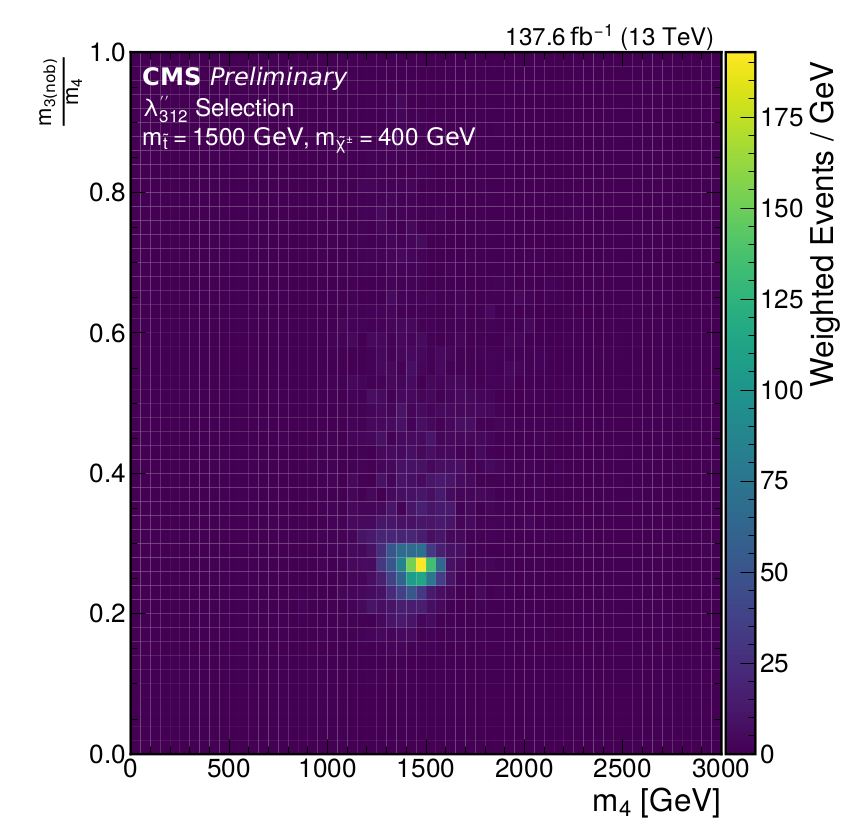
\includegraphics[width=0.35\textwidth]{figures/2D_peak}
  \end{center}
\end{frame}


\begin{frame}{Estimation Strategies}
  \begin{columns}
    \begin{halfcol}
      \begin{itemize}
      \item For all bump hunts, key technique is estimation of the background shape. 
      \item Traditional bump hunts have used ad-hoc functions \cite{zisopoulos_parametric_2023}, chosen because they approximate the observed shape. 
      \item However, this can introduce bias from the choice of function, and it has been shown that they scale poorly with increasing luminosity \cite{frate_modeling_2017}.
      \item For multidimensional searches, the problem can also be compounded by selecting a function for a potentially nontrivial 2D shape. 
      \end{itemize}
    \end{halfcol}

    \begin{halfcol}
      \begin{center}
        \graphiccite{figures/fit_table}{1}{zisopoulos_parametric_2023}
      \end{center}
    \end{halfcol}

  \end{columns}
\end{frame}

\begin{frame}{Current Strategy}
  \begin{itemize}
  \item We have implemented our background estimation using Gaussian process regression \cite{rasmussen_gaussian_2006}.
  \item This is non-parametric technique that reduces bias from the choice of parametric function.
  \item It has been shown to be robust against increasing luminosity\cite{frate_modeling_2017}.
  \item It is naturally extensible to multiple dimensions.
  \item Very well studied in statistics literature, and has a large number of well established implementations \cite{gardner_gpytorch_2021}. 
  \end{itemize}
\end{frame}

\section[Gaussian Process Regression]{Gaussian Process Regression Overview}
\label{sec:gauss-proc-regr}


\begin{frame}{Representing Histograms With Gaussians}
  \begin{itemize}
  \item We seek a way to describe our histogram probabilistically without reference to a specific parametric form. How can this be done?
  \item The answer: consider each of the N bins to be a random variable: part of a N-multivariate Gaussian (MVN).
  \item<1-> Consider our falling mass distribution.
  \item<2-> Imagine for simplicity we rebinned to have just 2 bins.
  \item<3-> We can represent the underlying distribution as a 2D Gaussian.
  \end{itemize}
  \begin{center}
    \begin{onlyenv}<1>
      \scalebox{0.5}{\includestandalone{\commonfiles{gp/histogram}}}
    \end{onlyenv}
    \def\meanOne{0.8}
    \def\meanTwo{0.4}
    \def\binOne{\meanOne}
    \def\binTwo{\meanTwo}
    \begin{onlyenv}<2>
      \scalebox{0.5}{\includestandalone{\commonfiles{gp/sampled_hist}}}
    \end{onlyenv}
    \foreach \one/\two [count=\n] in {\meanOne/\meanTwo, 0.6/0.2, 0.9/0.1} { %
      \pgfmathtruncatemacro\z{\n+2} %
      \only<\z>{ %
        \def\binOne{\one} %
        \def\binTwo{\two} %
        \scalebox{0.5}{\includestandalone{\commonfiles{gp/sampled_2d}}} %
        \scalebox{0.5}{\includestandalone{\commonfiles{gp/sampled_hist}}}} %
    }
  \end{center}
\end{frame}

\begin{frame}{Prediction}
  \begin{itemize}
  \item The previous slide shows how we can use a MVN to describe a histogram.
  \item How can we have actual predictive power? How can we incorporate known data to extrapolate to unknown points?
  \item Answer: Condition the gaussian! If $p(b_{1},b_{2}) \sim \mathcal{N}(b_{1},b_{2})$ then $p(b_{1} | b_{2,obs} ) \sim  \mathcal{N}(b_{1},b_{2,obs})$
  \end{itemize}
  \begin{center}
    \def\meanOne{0.8}
    \def\meanTwo{0.4}
    \def\binOne{0.7}
    \def\binTwo{0.48}
    \def\binTwoStd{0.1}
    \scalebox{0.5}{\includestandalone{\commonfiles{gp/conditioned_2d}}} %
    \scalebox{0.5}{\includestandalone{\commonfiles{gp/conditioned_hist}}} %
  \end{center}
  
\end{frame}


\begin{frame}{Beyond the Histogram}
  \begin{itemize}
  \item The remaining question:
  \item What if we have more than 2 bins? What if we have infinitely many bins (ie a function)?
  \item How should we describe the MVN then?
  \end{itemize}
\end{frame}

\begin{frame}{What is a Gaussian Process?}
  \begin{definition}
    A gaussian process is a possibly infinite series of random variables, any finite subset of which is jointly gaussian.
  \end{definition}


  Generall, the random variables are indexed by real values $x$, since we are generally considering regression over $\mathbb{R}^{n}$.


  A gaussian process $f(x)$ is is completely defined by its mean and covariance
  \begin{equation}
    \begin{split}
      \markpos{gpmean}{m(x)} &= \mathbb{E} \left[ f(x) \right] \\
      \markpos{gpk}{k(x,x')} &= \mathbb{E} \left[ \left( f(x) - m(x) \right)  \left( f(x') - m(x') \right)\right] 
    \end{split}
  \end{equation}


  \begin{center}
    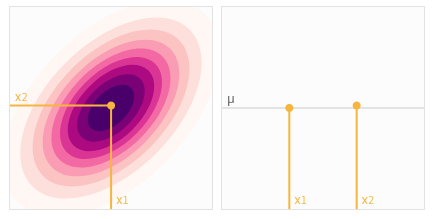
\includegraphics[width=0.4\textwidth]{figures/two_points_1}
    \hspace{1cm}
    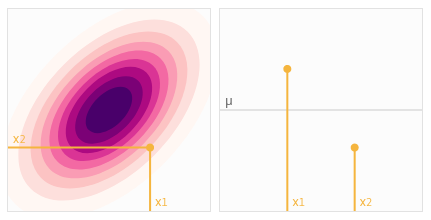
\includegraphics[width=0.4\textwidth]{figures/two_points_2}
  \end{center}

  \begin{onlyenv}<2>
    \posannot{gpmean}{fill=UMNMaroon!10, draw=UMNMaroon}{The mean value of the MVN.}
    \posannot[-30:4cm]{gpk}{fill=UMNMaroon!10, draw=UMNMaroon}{The covariance between  any two points. \\For any collection of points the the covariance matrix is $K_{ij} = k(x_{i},x_{j})$.}
  \end{onlyenv}
\end{frame}

% \begin{frame}{Gaussian Process Regression}
%   \begin{itemize}
%   \item The ability to define distributions over functions allows us to do inference using Baye's theorem. 
%   \item Specifically, given $N$ training points and a Gaussian process prior, we can produce a posterior Gaussian process that provides a means to do regression. 
%   \end{itemize}
%   \begin{center}
%     \graphiccite{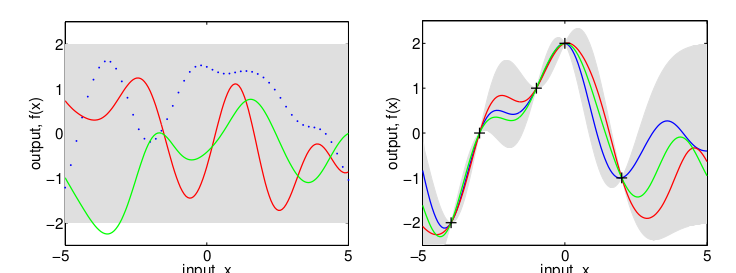
\includegraphics[width=0.7\textwidth]{figures/prior_and_conditioning}}{\cite{rasmussen_gaussian_2006}}
%   \end{center}
% \end{frame}

\begin{frame}{Kernels}
  \begin{itemize}
  \item The choice of kernel is the most important aspect of Gaussian processes. 
  \item The choice of $k(x,y)$ reflects different understandings of how the points should be correlated, how smooth the functions should be, etc. 
  \item The choice of kernel consists of both the selection of the form and the hyperparameters. 
    \begin{itemize}
    \item The kernel form is chosen based on the properties of the problem at hand.
    \item The hyperparameters are chosen to optimize the evidence. 
    \end{itemize}
  \end{itemize}

  \begin{align}
    \log p(\bm{y}|X) =
    \markpos{term1}{-\frac{1}{2}\bm{y}^T(K+\sigma^2_n I)^{-1}\bm{y}}
    - \markpos{term2}{\frac{1}{2}\log|K+\sigma^2_n I|}
    - \frac{n}{2}\log2\pi
  \end{align}
  \begin{center}
    \graphiccite{figures/different_scale}{0.4}{rasmussen_gaussian_2006}
  \end{center}
  \begin{onlyenv}<2>
    \posannot{term1}{fill=UMNMaroon!10, draw=UMNMaroon}{Compatibility of model with data}
    \posannot[210:3cm]{term2}{fill=UMNMaroon!10, draw=UMNMaroon}{Overfitting penalty works against kernels with large determinants.}
  \end{onlyenv}
\end{frame}


\section[GPR Result]{GPR For Combinatorial Backgrounds}
\label{sec:2d-gauss-proc}

\begin{frame}{Kernels in 2D}
  \begin{itemize}
  \item Show simplest RBF Kernel
  \item Show GRBF kernel
  \item Show NN kernel
  \end{itemize}

  SHOW IMAGES HERE OF WHAT THE DIFFERENT KERNELS LOOK LIKE
\end{frame}


\begin{frame}{Overview}
  \begin{itemize}
  \item We use GP regression to estimate backgrounds in both one and two dimensional searches.
  \item In both cases, we mask the region of space where the signal is expected, then use regression to estimate the background in the masked region.
  \item Use both simulation and control region data to study efficacy of different methods. 
  \item Majority of studies have been focused on kernel selection and approximation techniques.
  \end{itemize}

  \begin{center}
    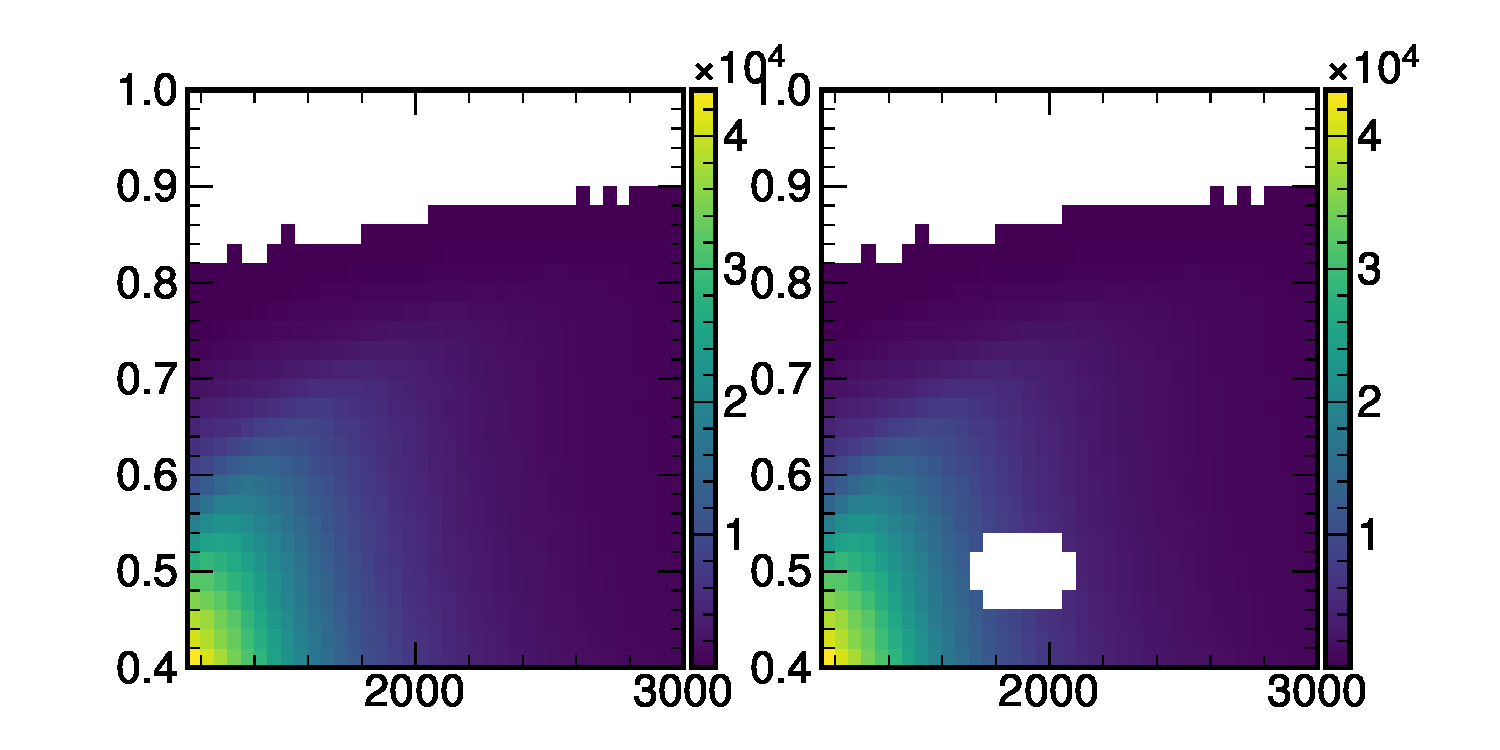
\includegraphics[width=0.7\textwidth]{figures/example_masking}
  \end{center}
\end{frame}

\begin{frame}{2D Results}
  \begin{itemize}
  \item We see promising results for estimation in windows of varying sizes over the 2D plane. 
  \item Depending on region, either generalized RBF kernels or and RBF kernel supplemented with the deep network have shown promising and robust estimative abilities.
  \end{itemize}

  \begin{center}
    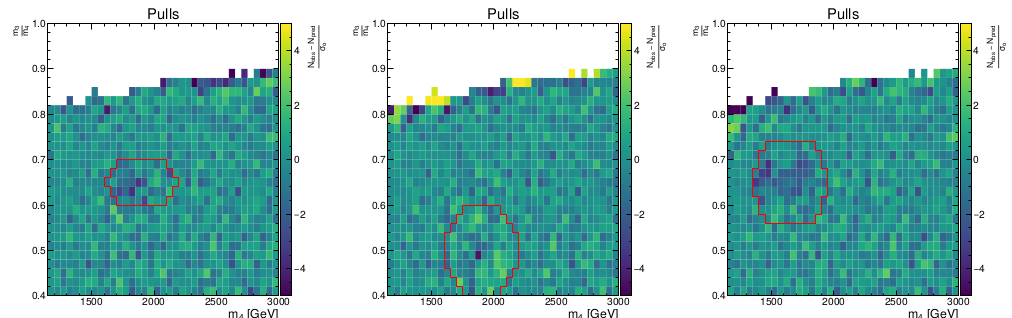
\includegraphics[width=\textwidth]{figures/nn_results_1} 
  \end{center}
\end{frame}

\begin{frame}{Fit Using Inhomegenous RBF}
  \begin{center}
    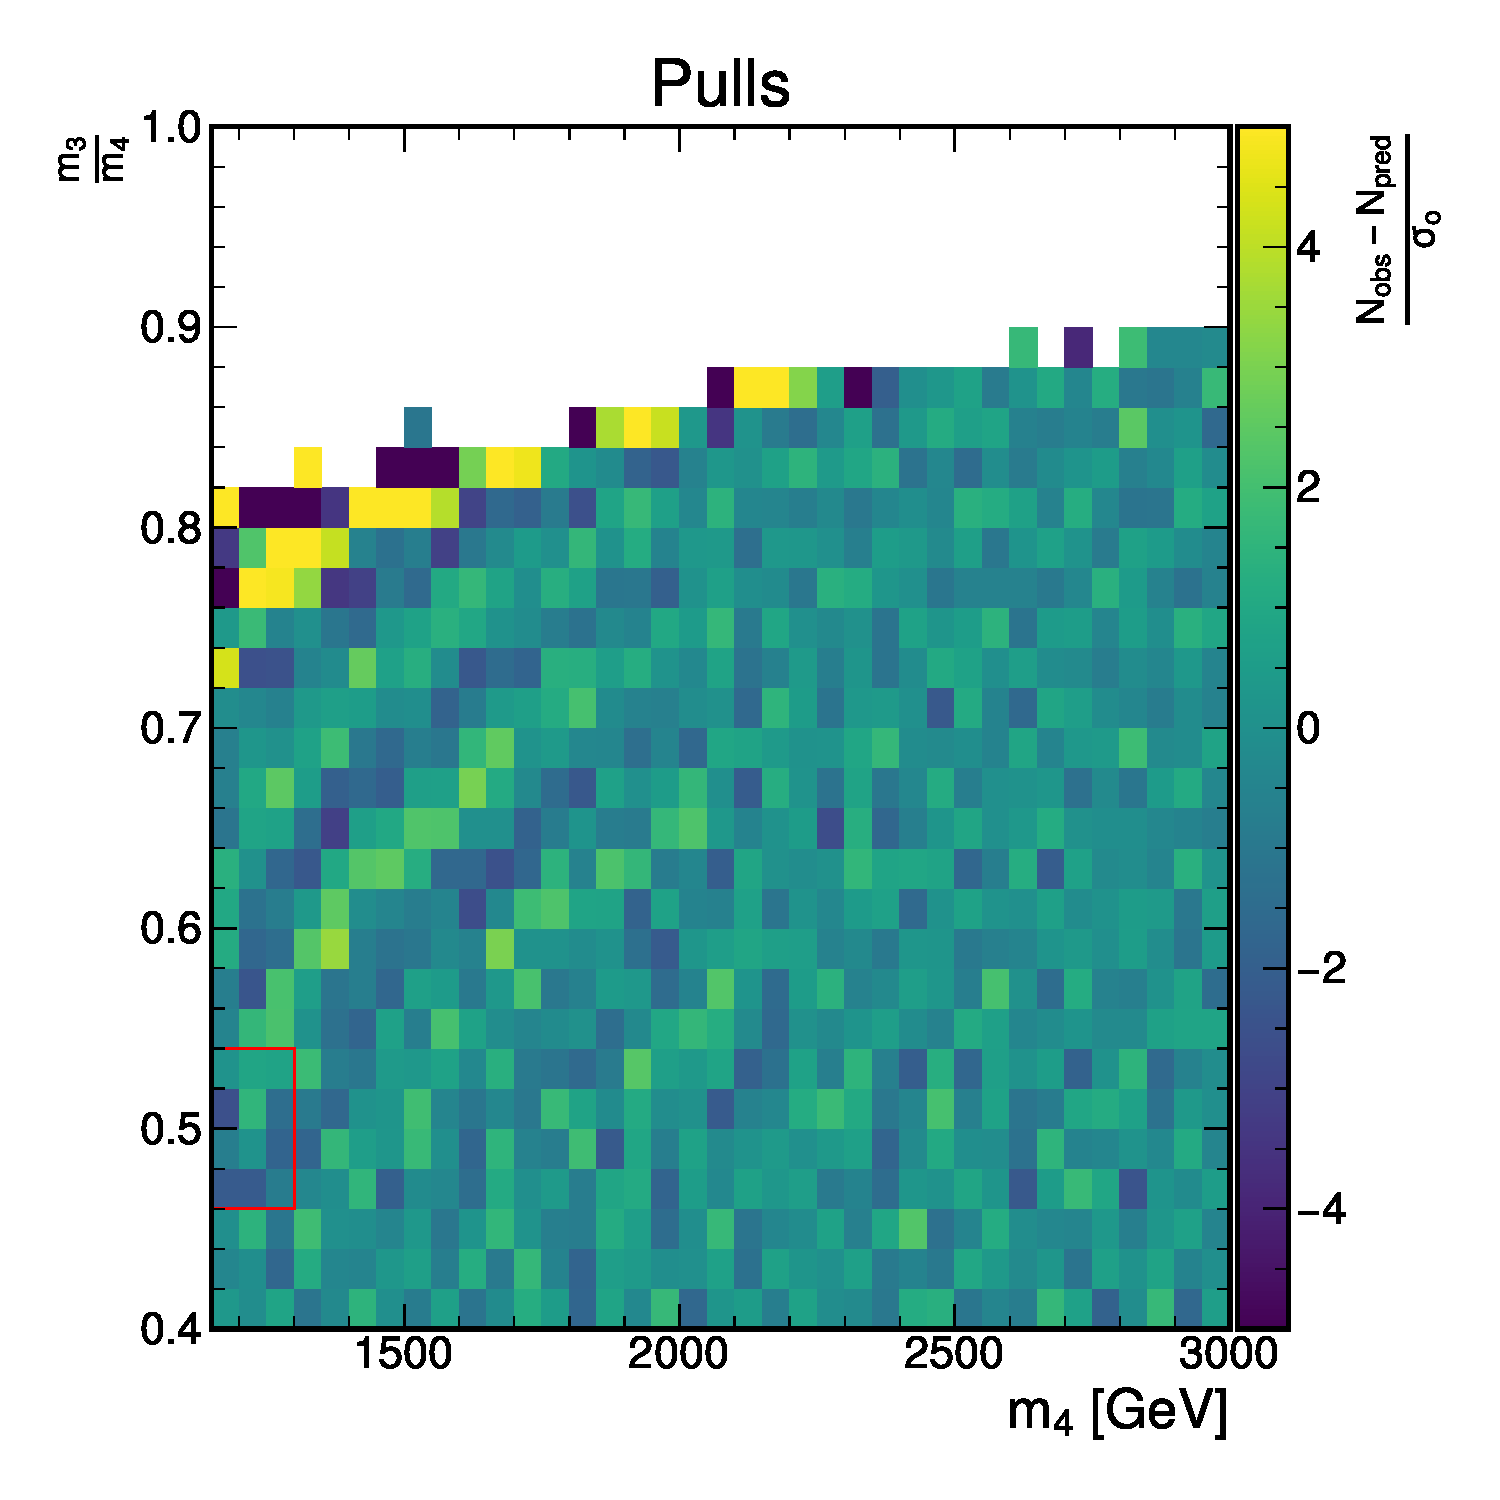
\includegraphics[width=0.3\textwidth]{figures/2dpullplots/rbf/E_1200_0p5_100_0p05.pdf} 
    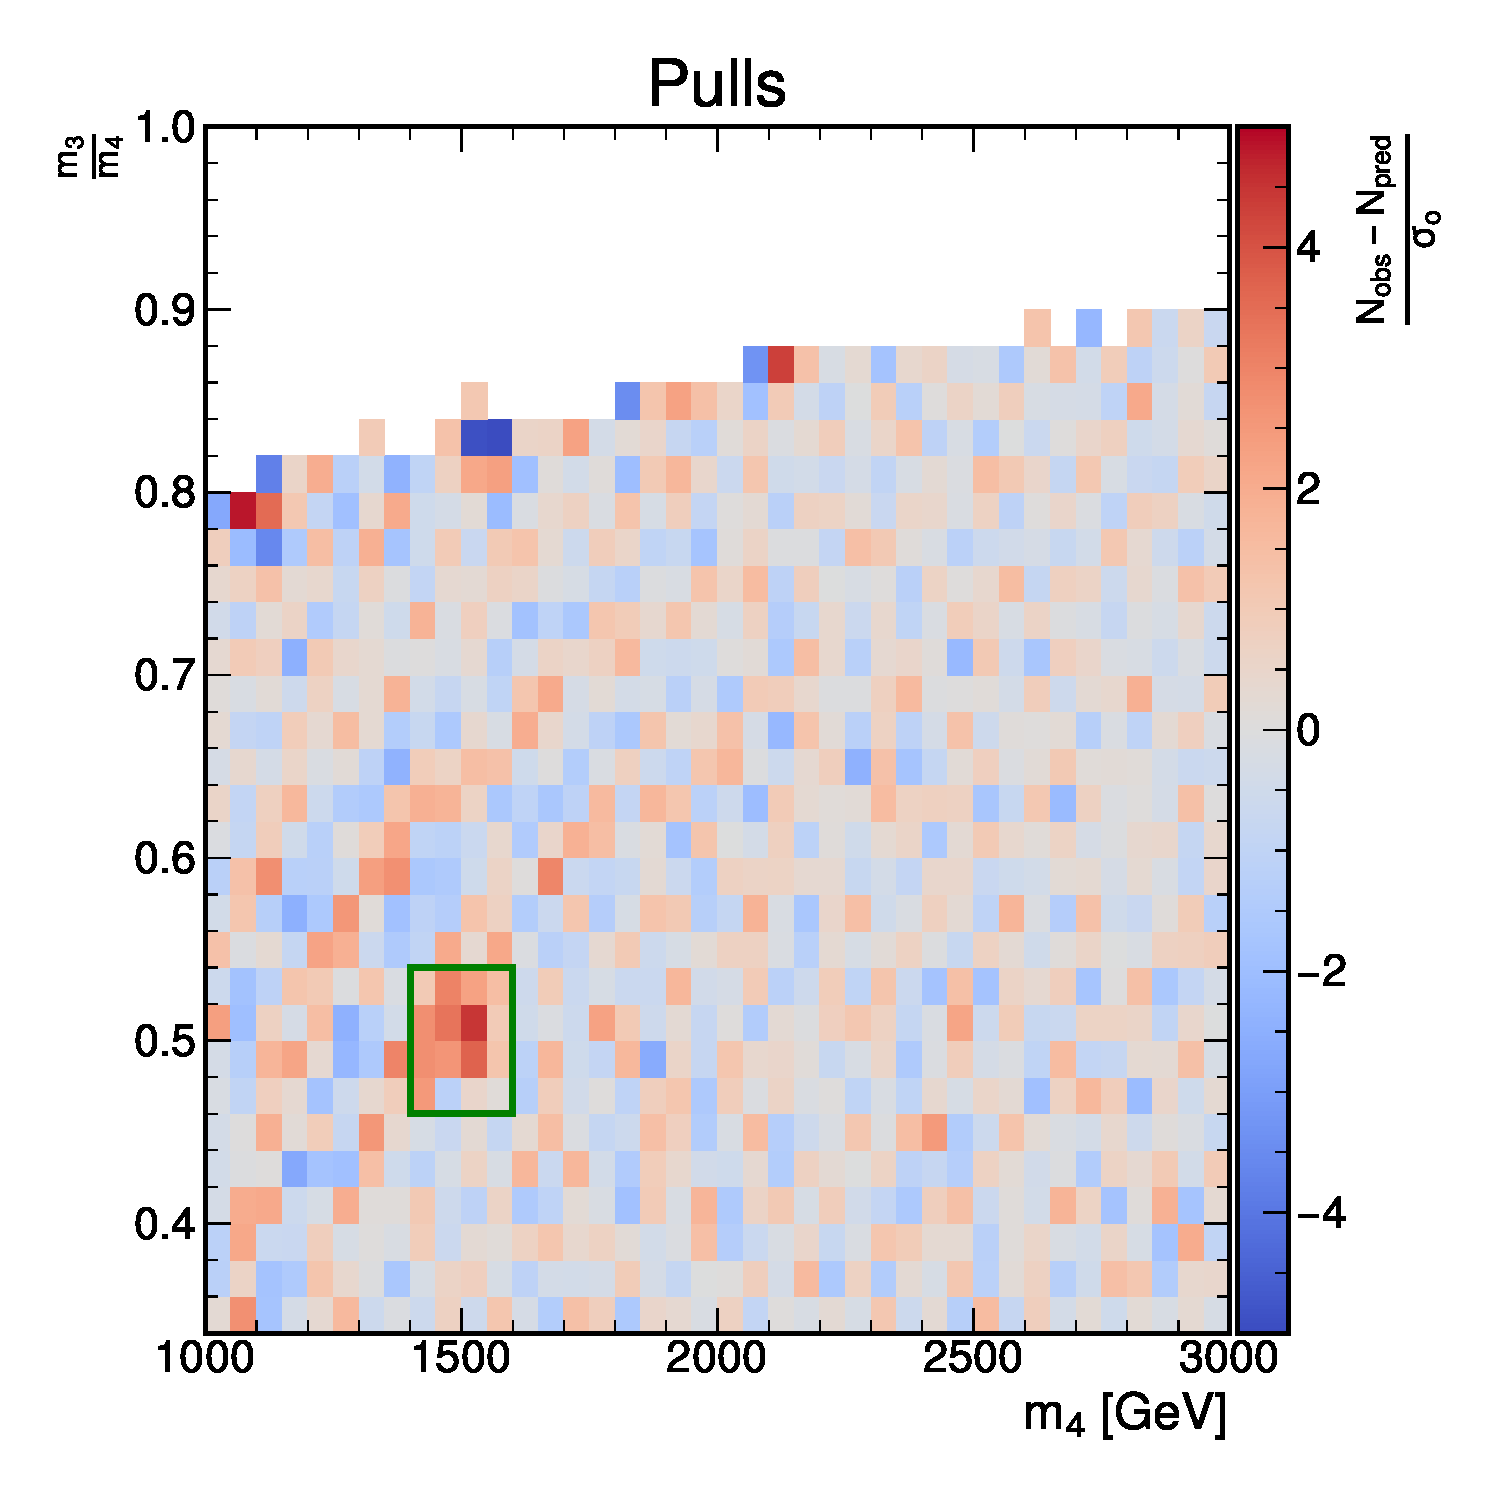
\includegraphics[width=0.3\textwidth]{figures/2dpullplots/rbf/E_1500_0p5_100_0p05.pdf} 
    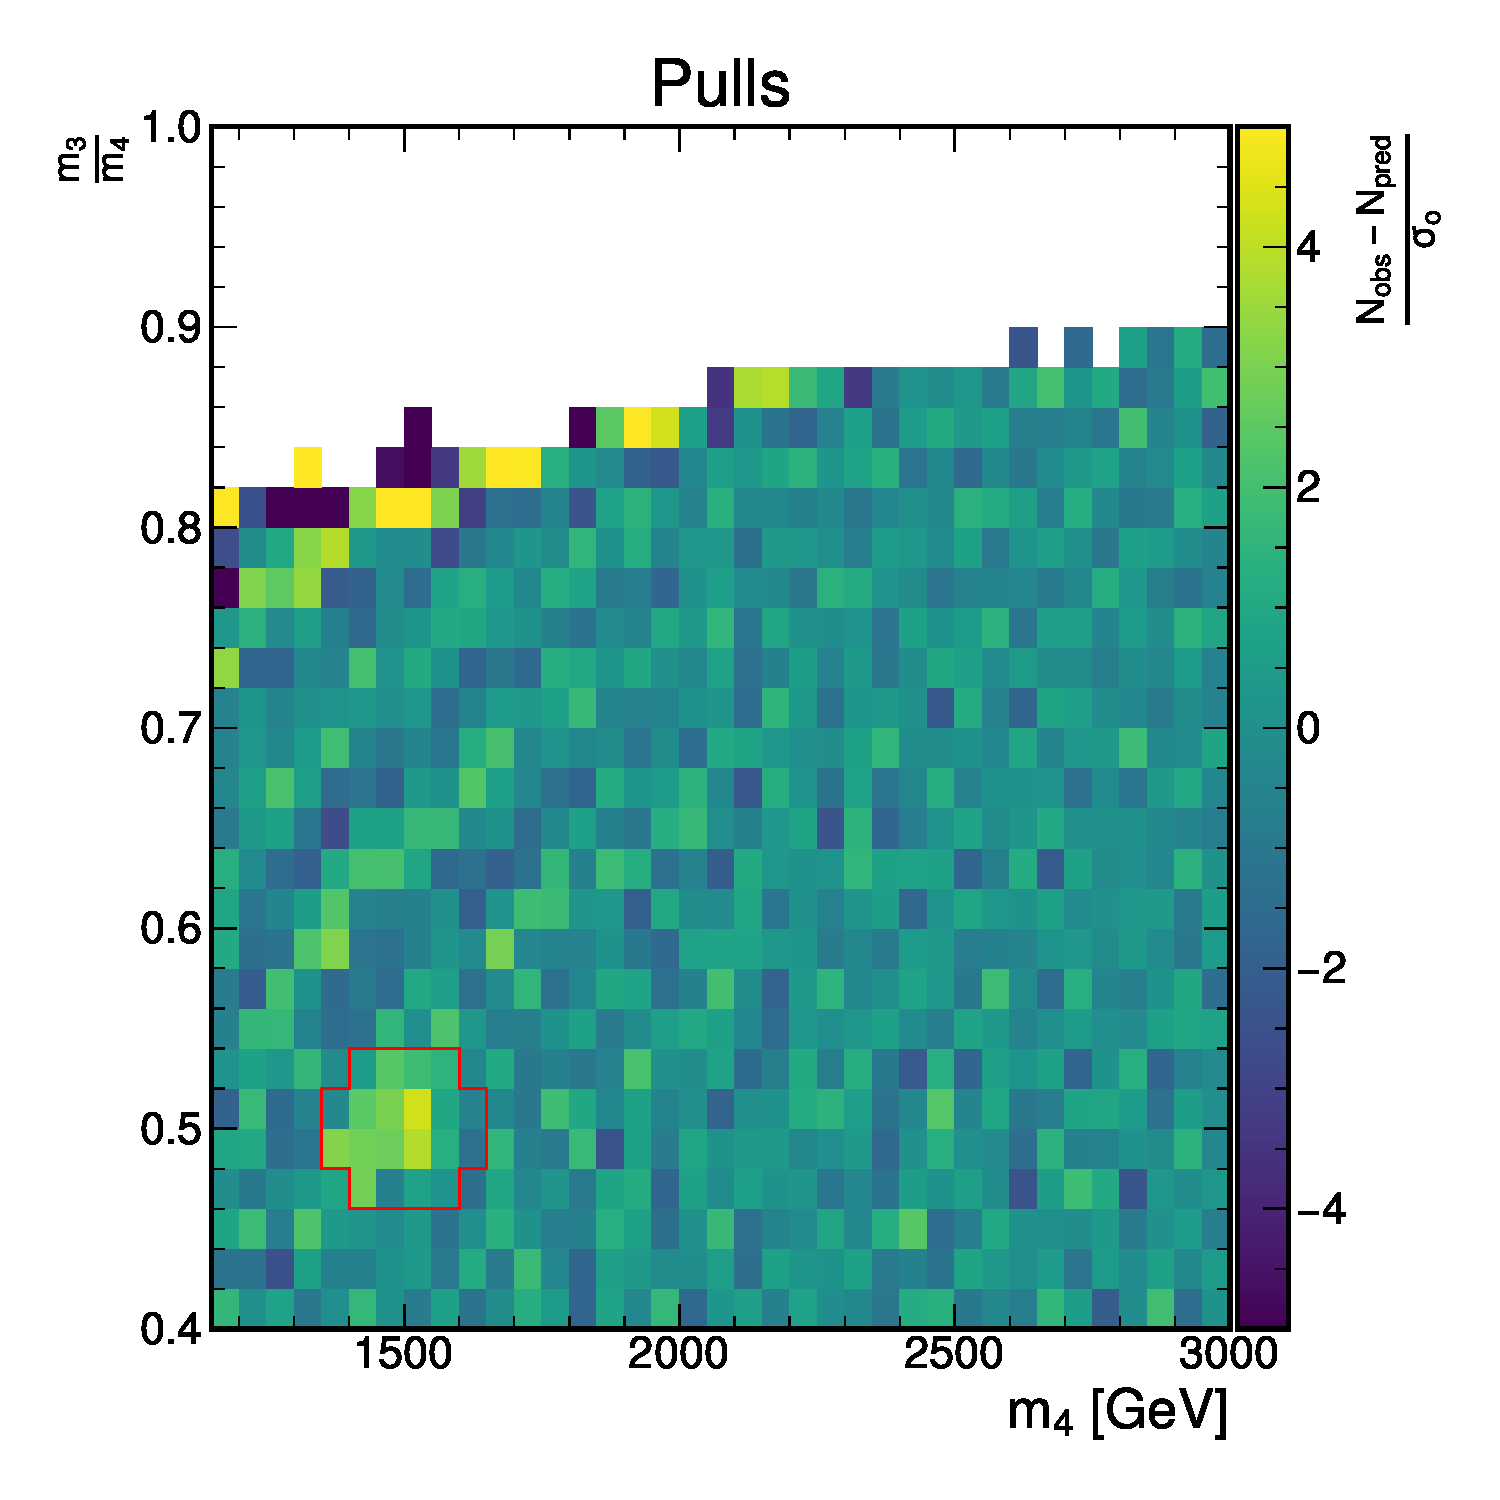
\includegraphics[width=0.3\textwidth]{figures/2dpullplots/rbf/E_1500_0p5_150_0p05.pdf} 
    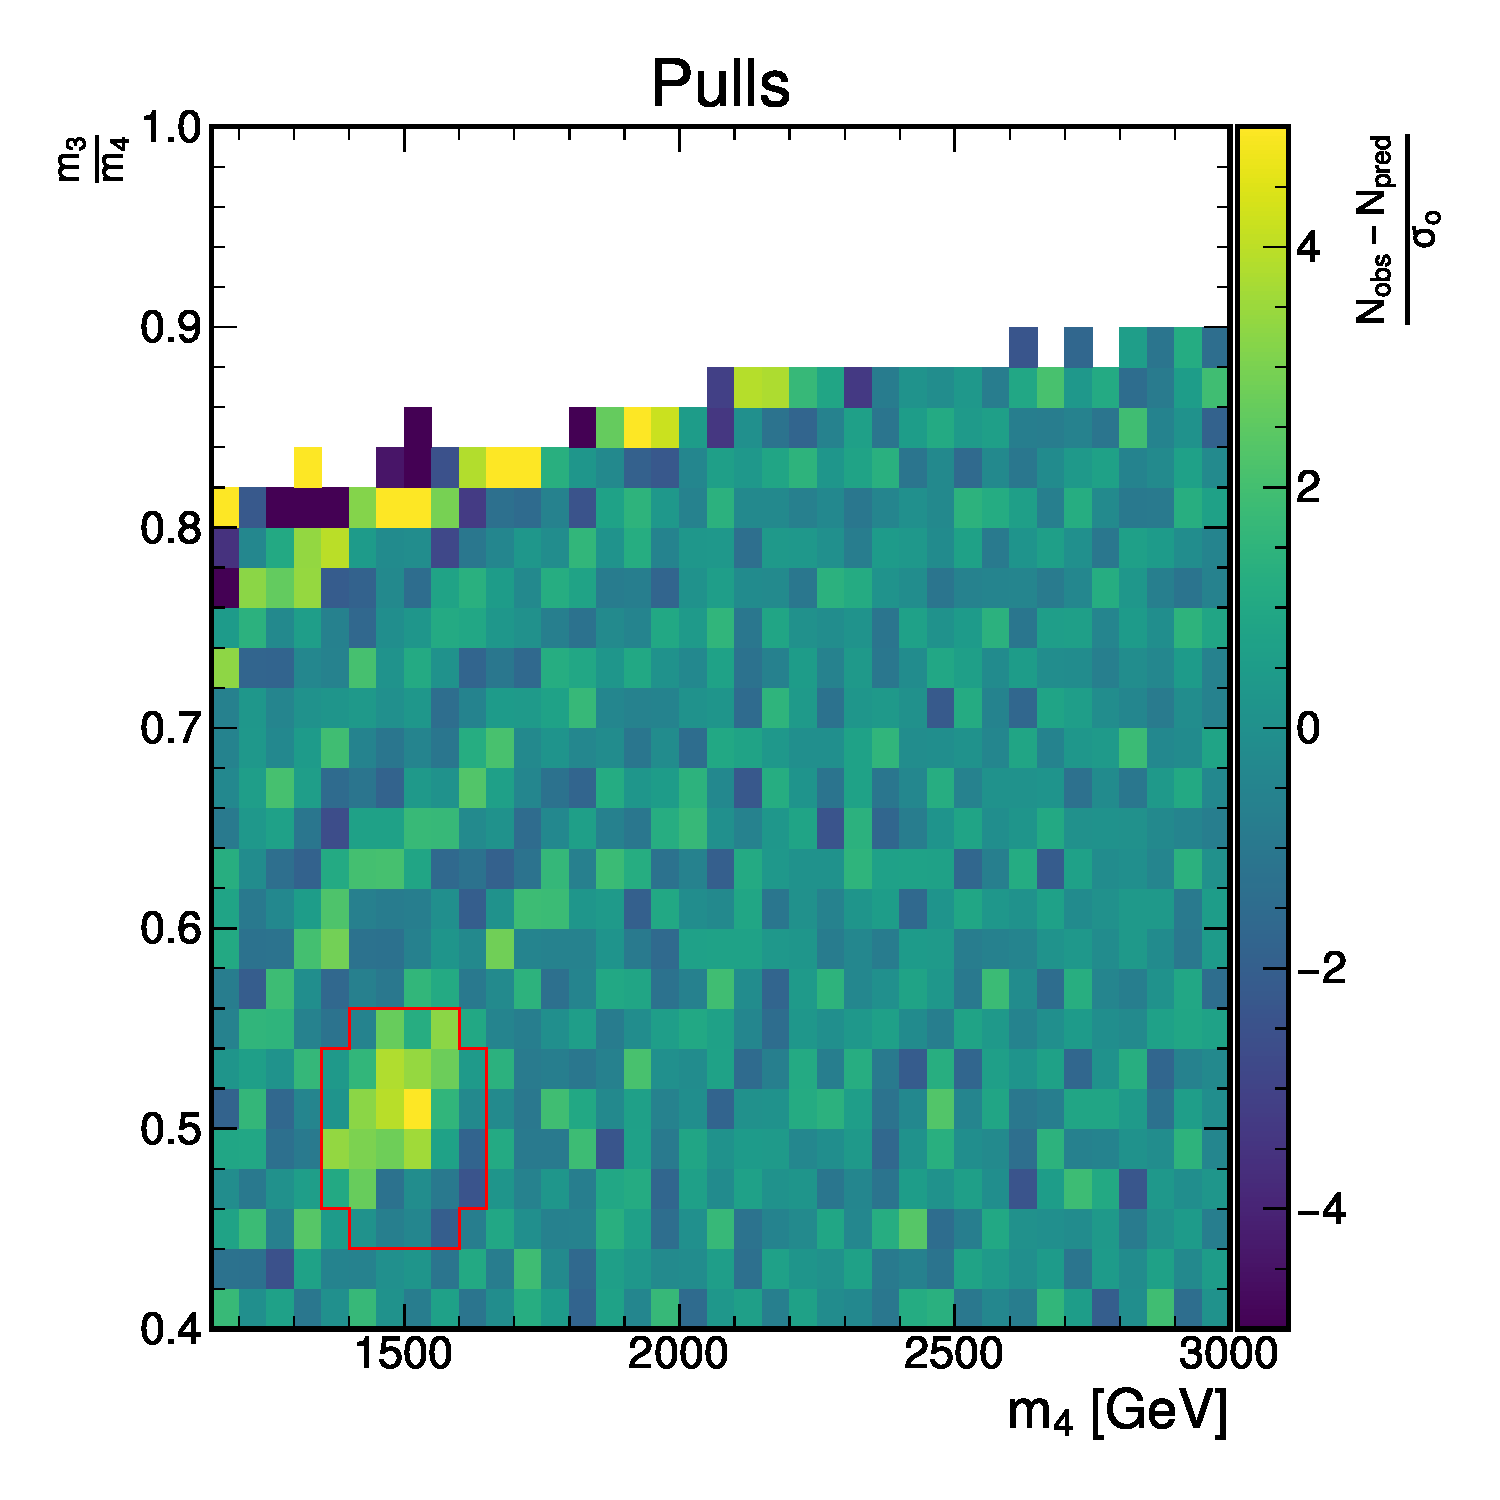
\includegraphics[width=0.3\textwidth]{figures/2dpullplots/rbf/E_1500_0p5_150_0p07.pdf} 
    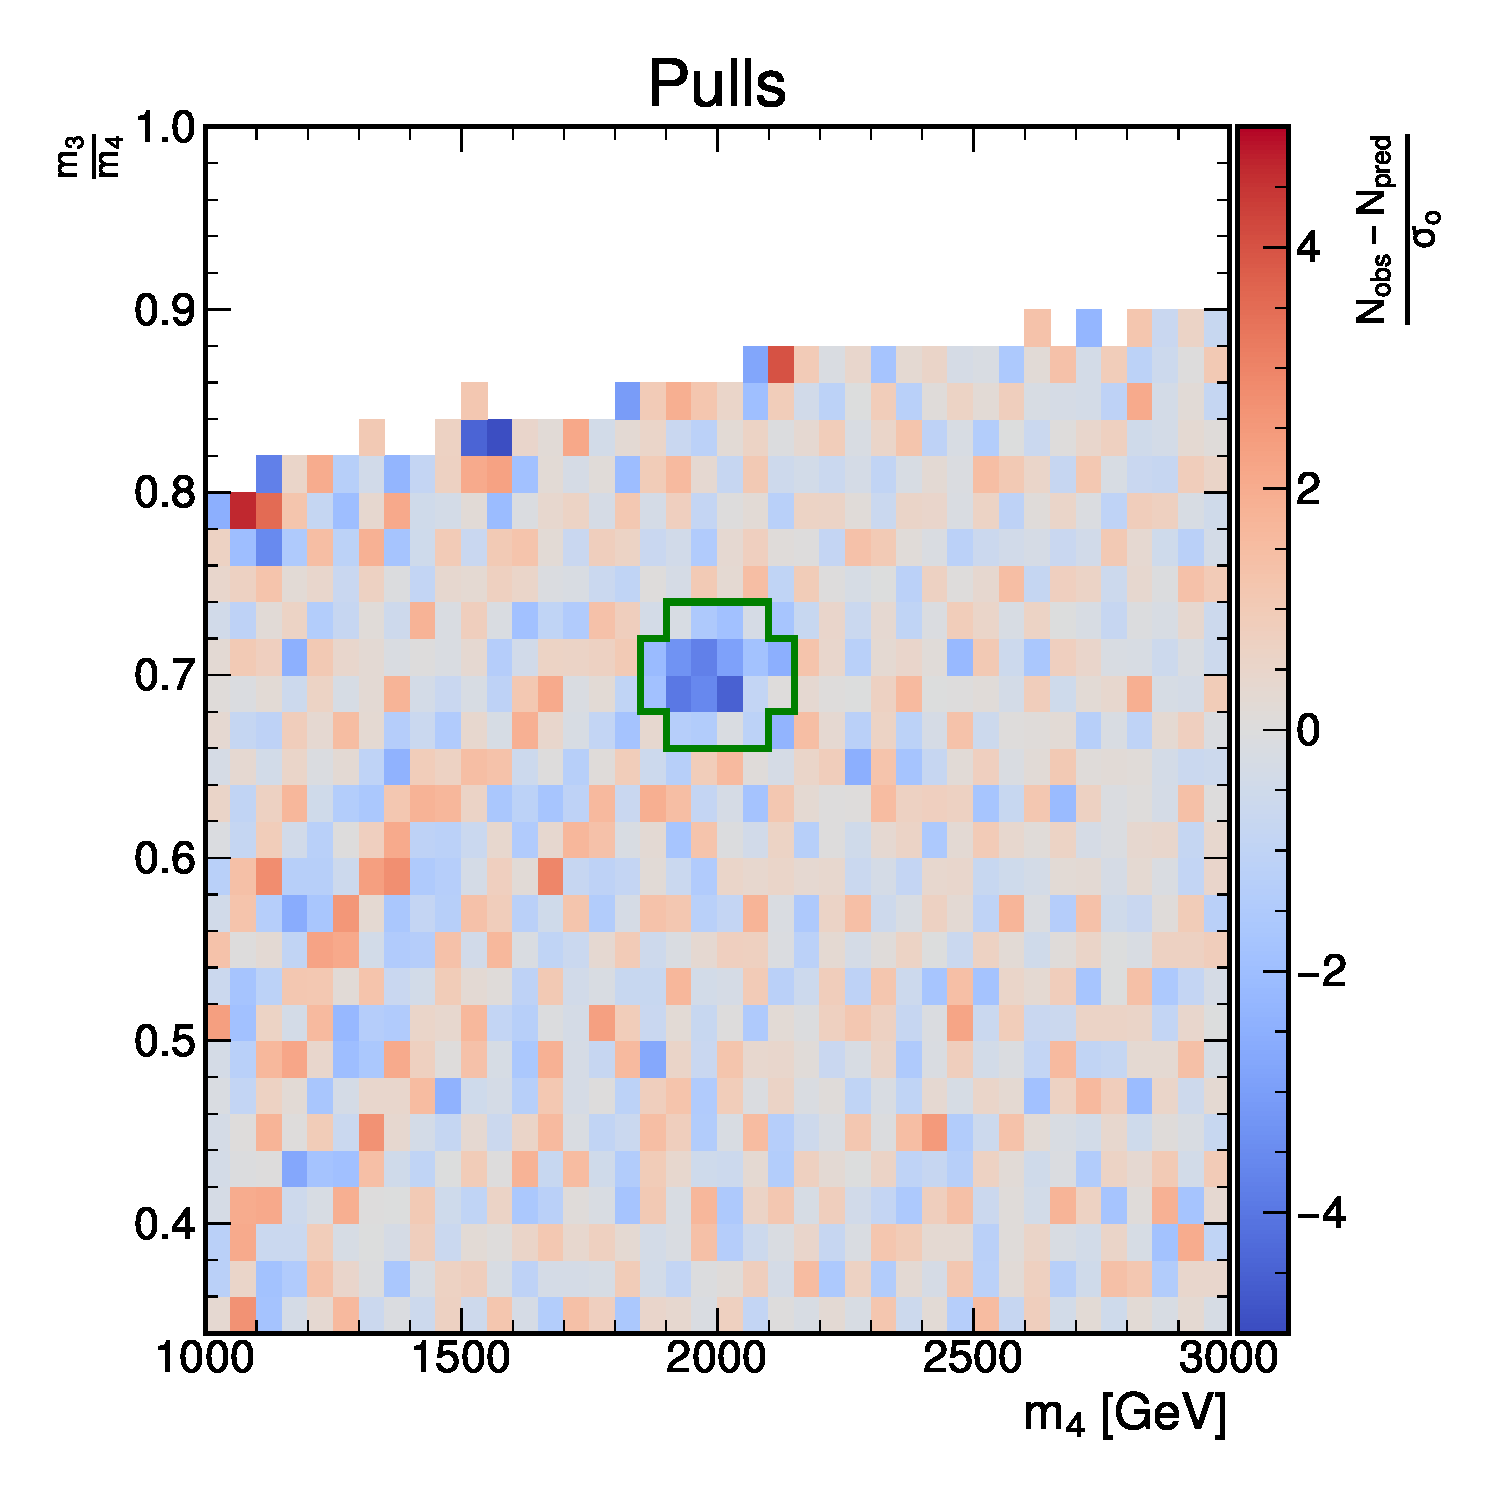
\includegraphics[width=0.3\textwidth]{figures/2dpullplots/rbf/E_2000_0p7_150_0p05.pdf} 
    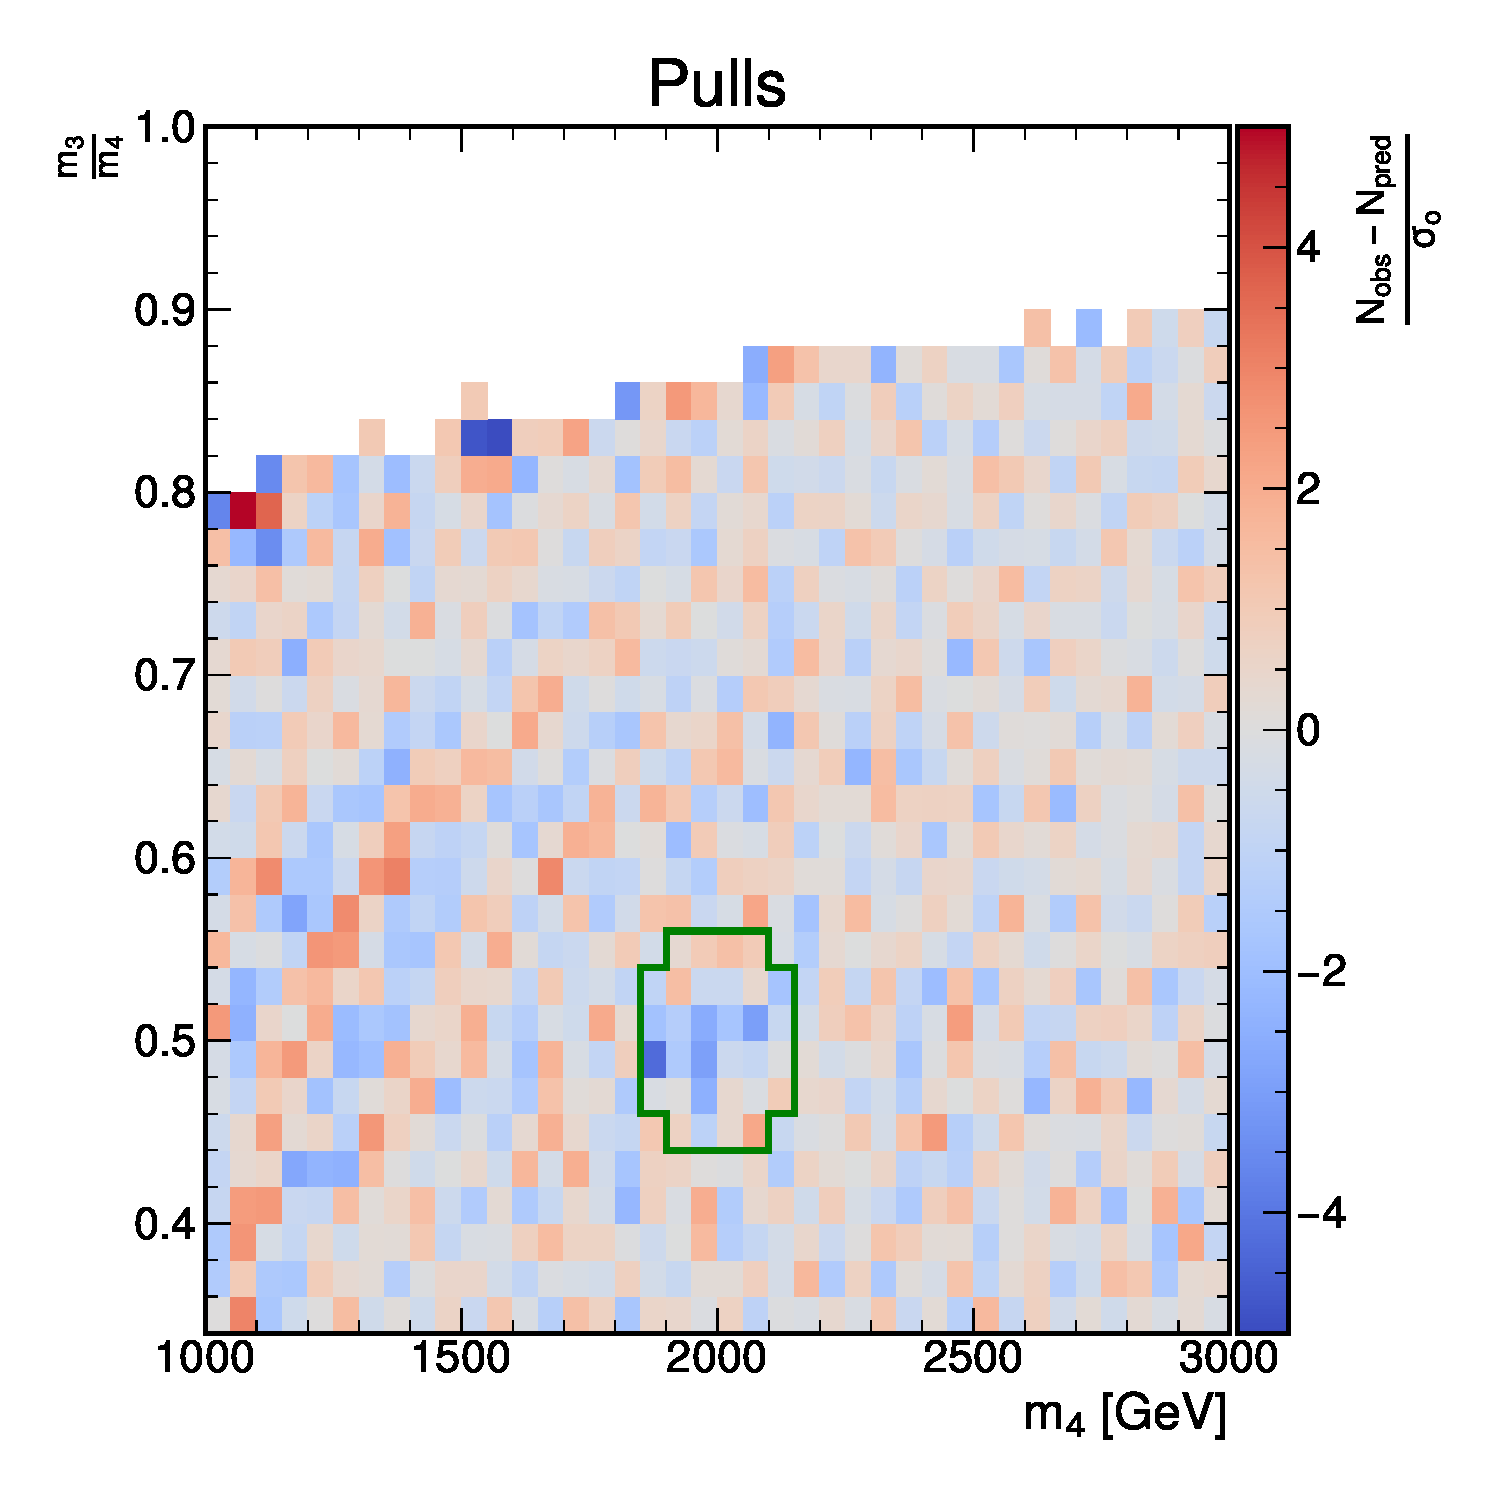
\includegraphics[width=0.3\textwidth]{figures/2dpullplots/rbf/E_2000_0p5_150_0p07.pdf} 
  \end{center}
  %\begin{center}
  %  \begin{annotimage}{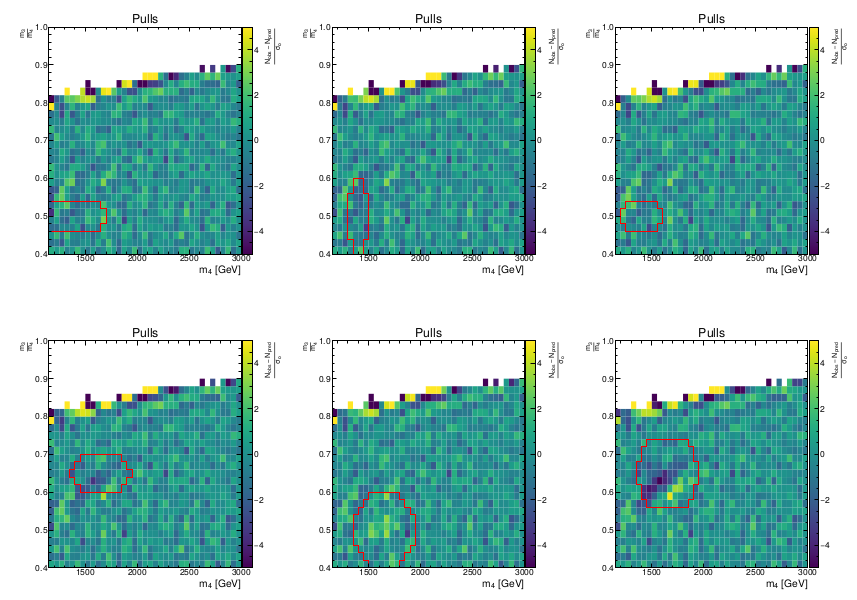
\includegraphics[width=0.85\textwidth]{figures/grbf_results}}
  %    \draw[thick,red, -latex] (1,0.5) node[black, align=center, anchor=west] {{\tiny Challenging area for RBF}} -- (0.8,0.22);
  %  \end{annotimage}
  %\end{center}
\end{frame}

\begin{frame}{Fit Using GRBF}
  \begin{center}
    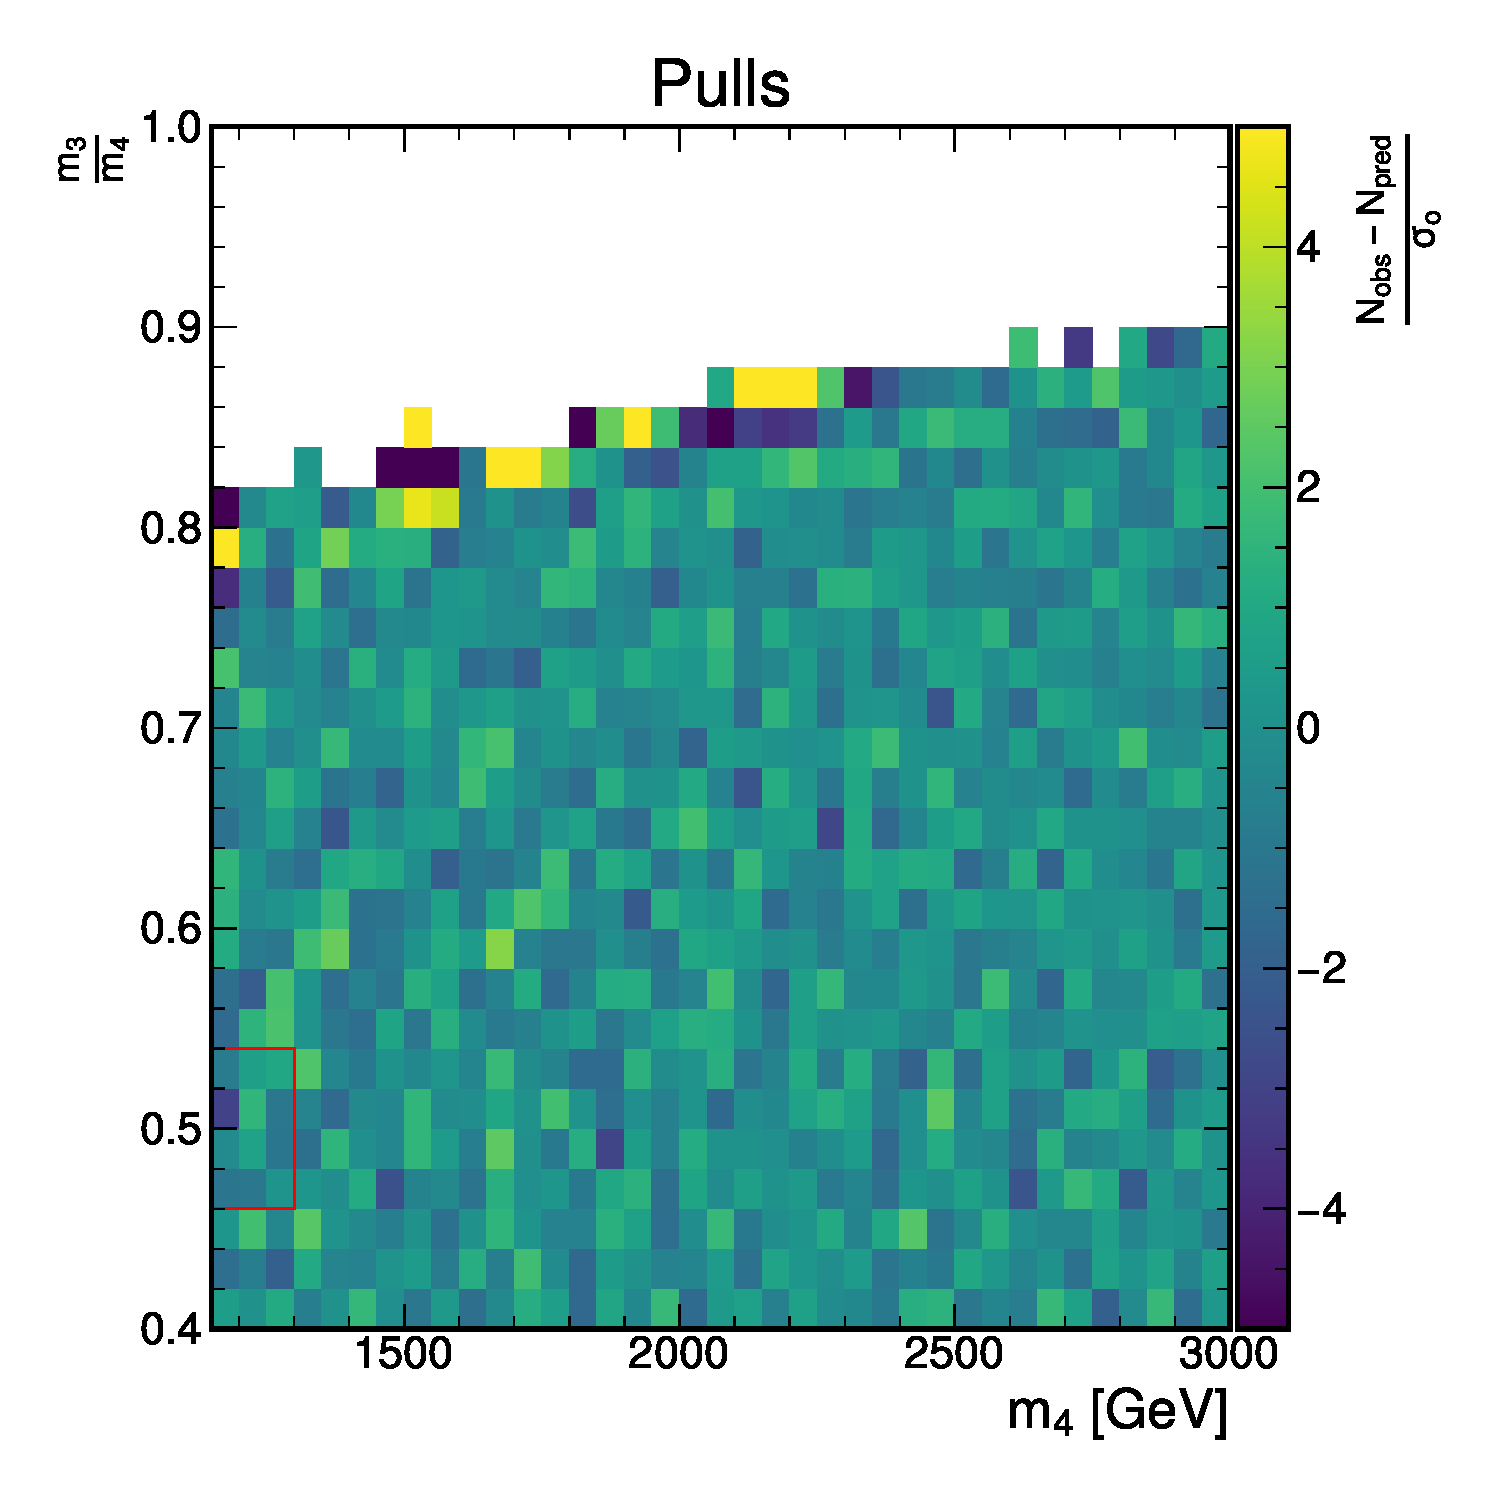
\includegraphics[width=0.3\textwidth]{figures/2dpullplots/grbf/E_1200_0p5_100_0p05.pdf} 
    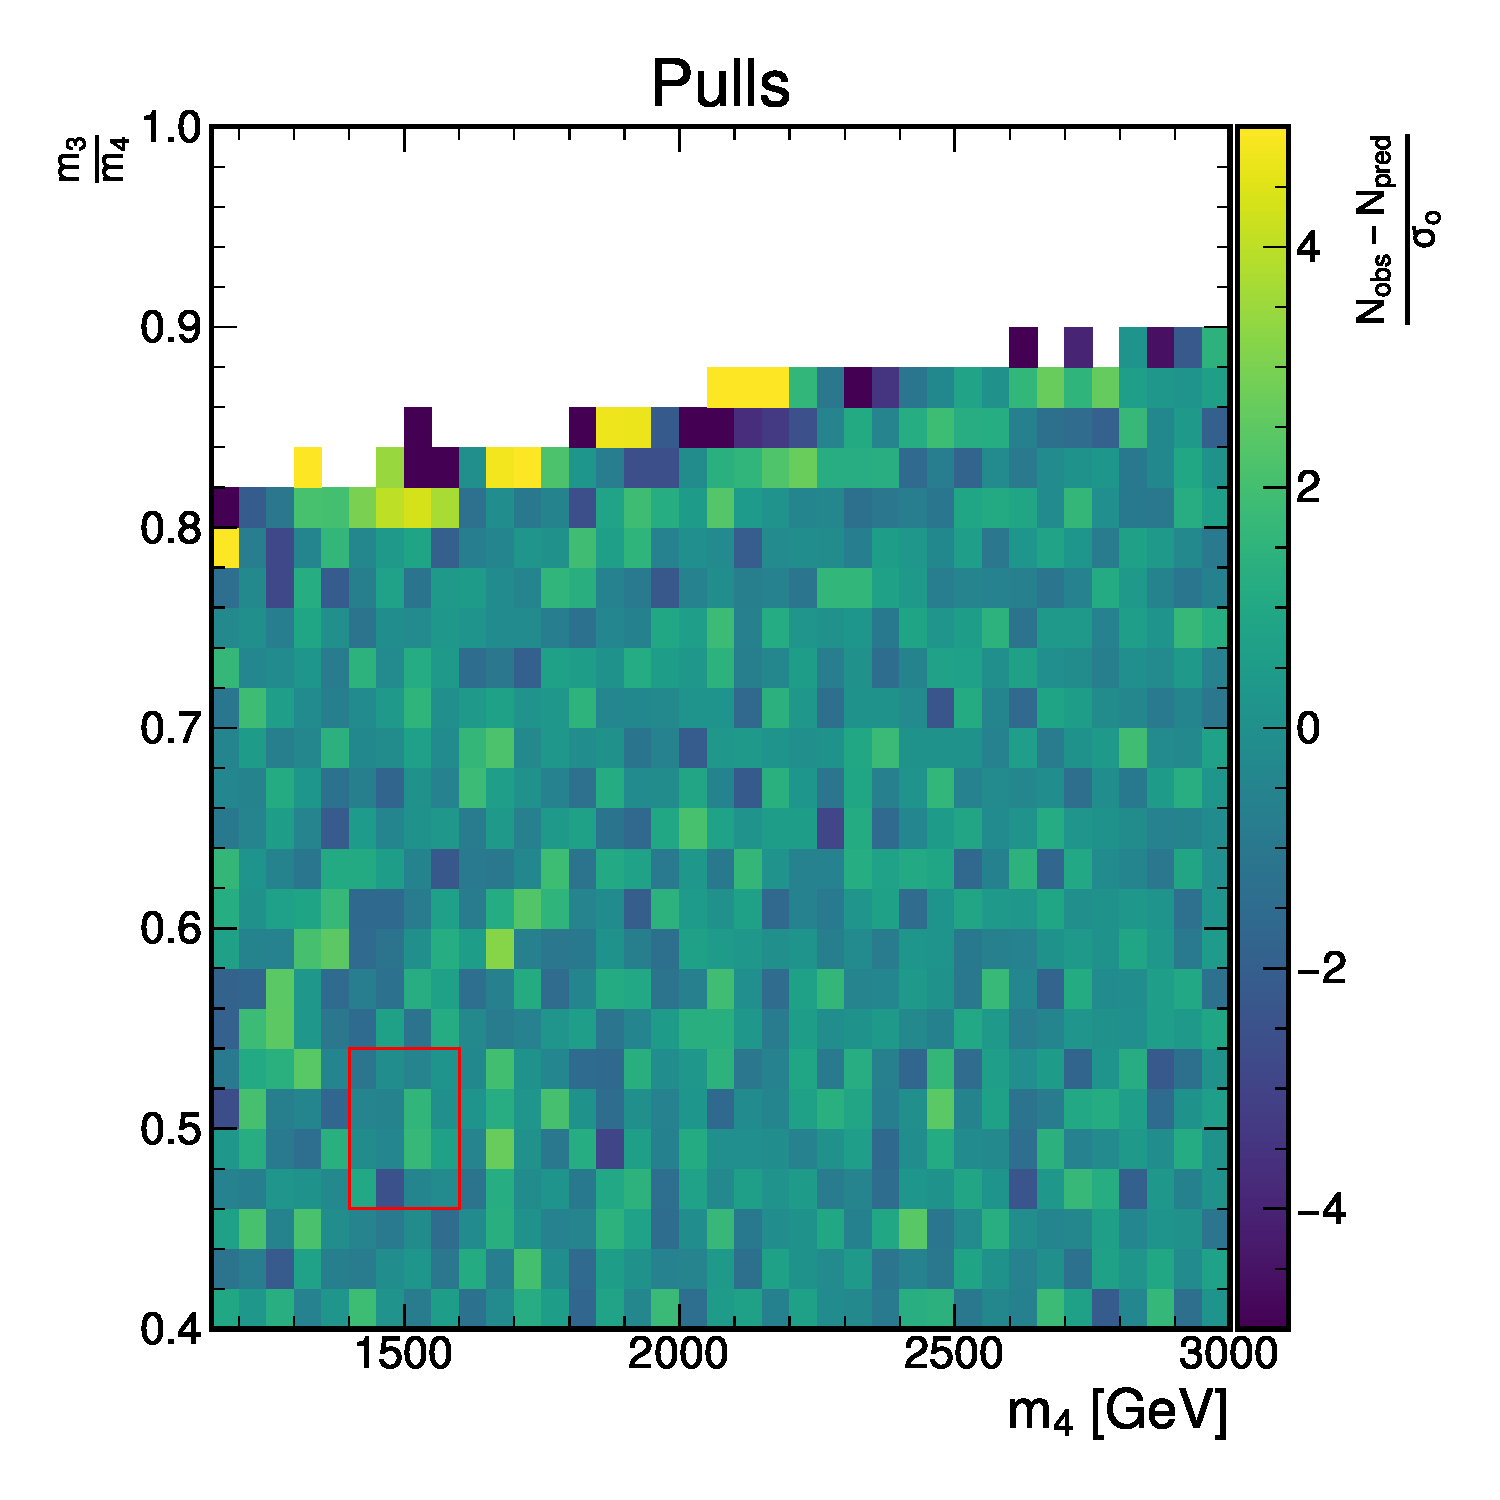
\includegraphics[width=0.3\textwidth]{figures/2dpullplots/grbf/E_1500_0p5_100_0p05.pdf} 
    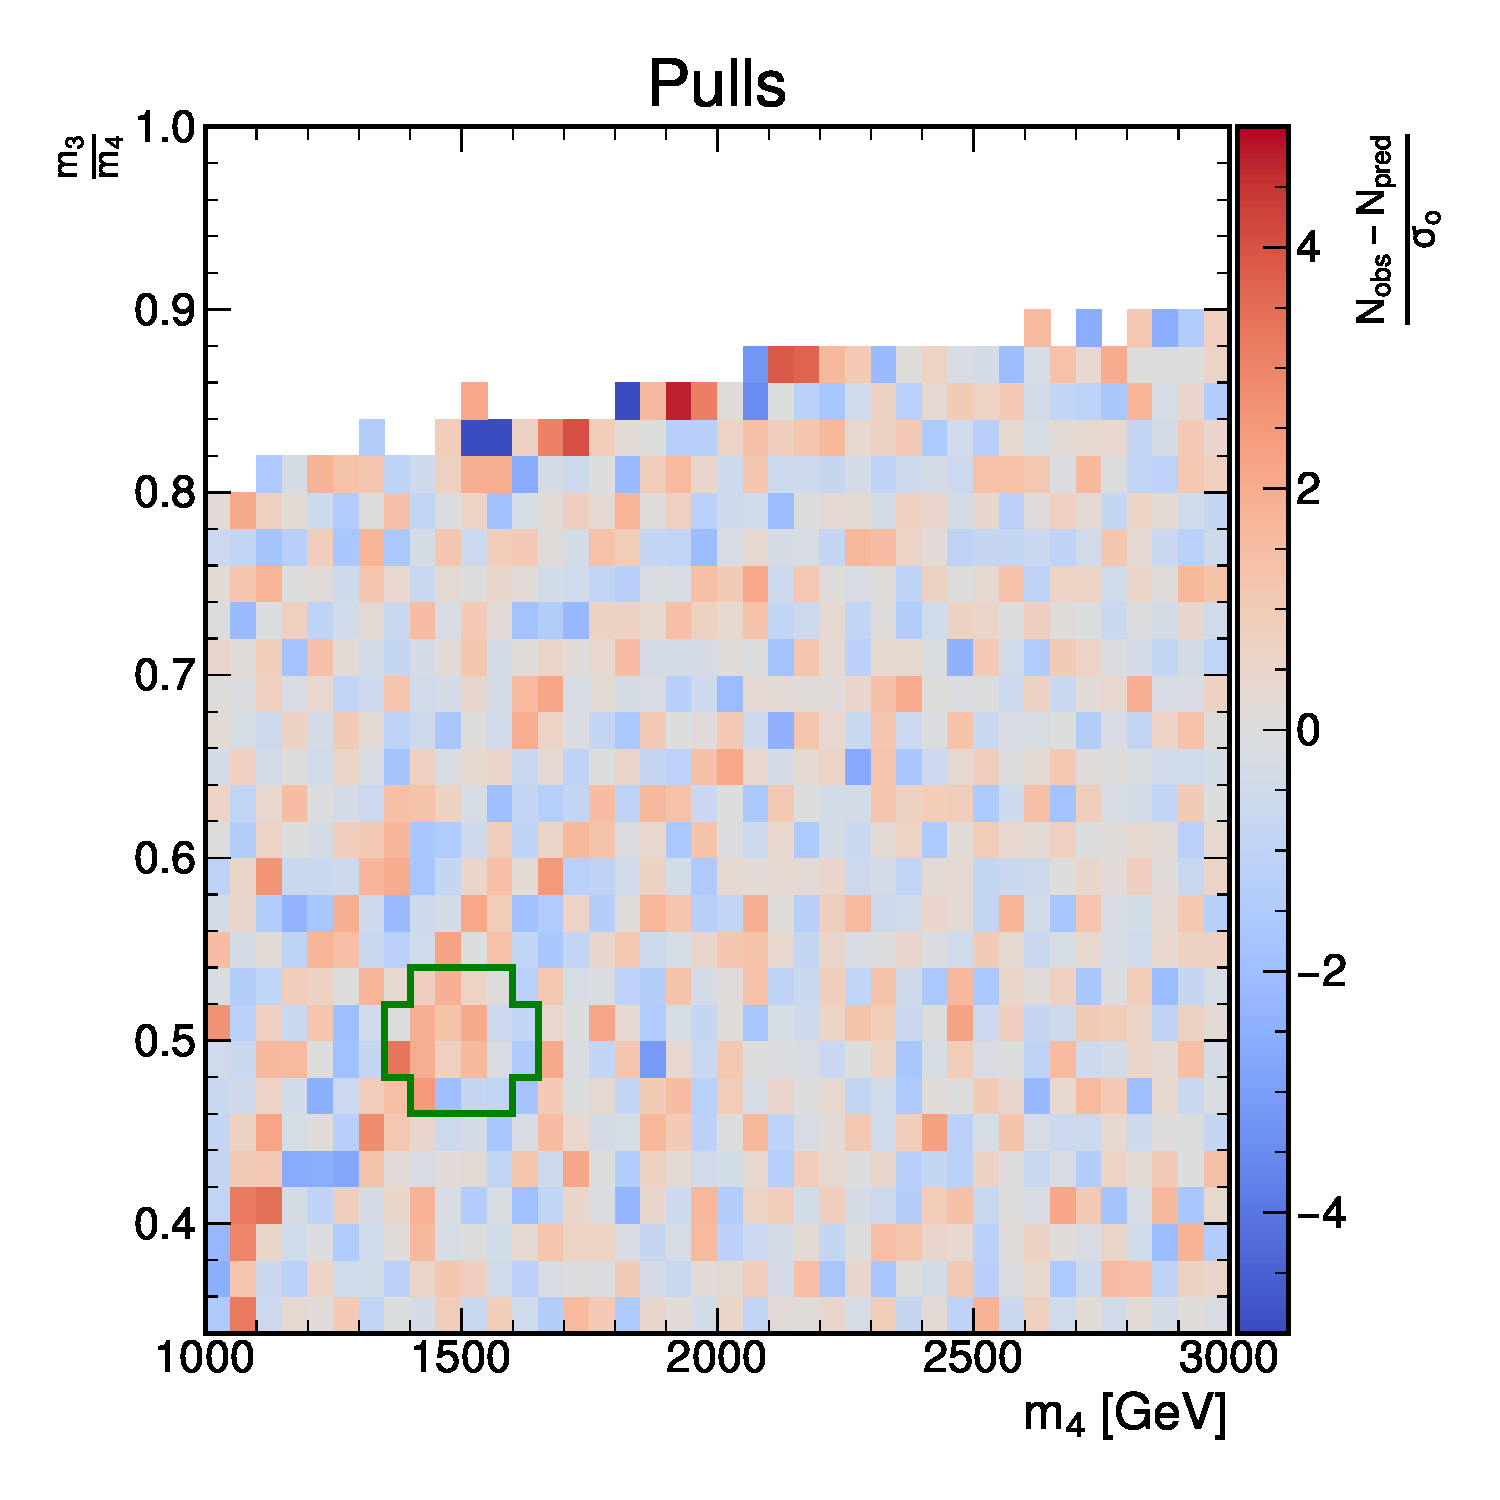
\includegraphics[width=0.3\textwidth]{figures/2dpullplots/grbf/E_1500_0p5_150_0p05.pdf} 
    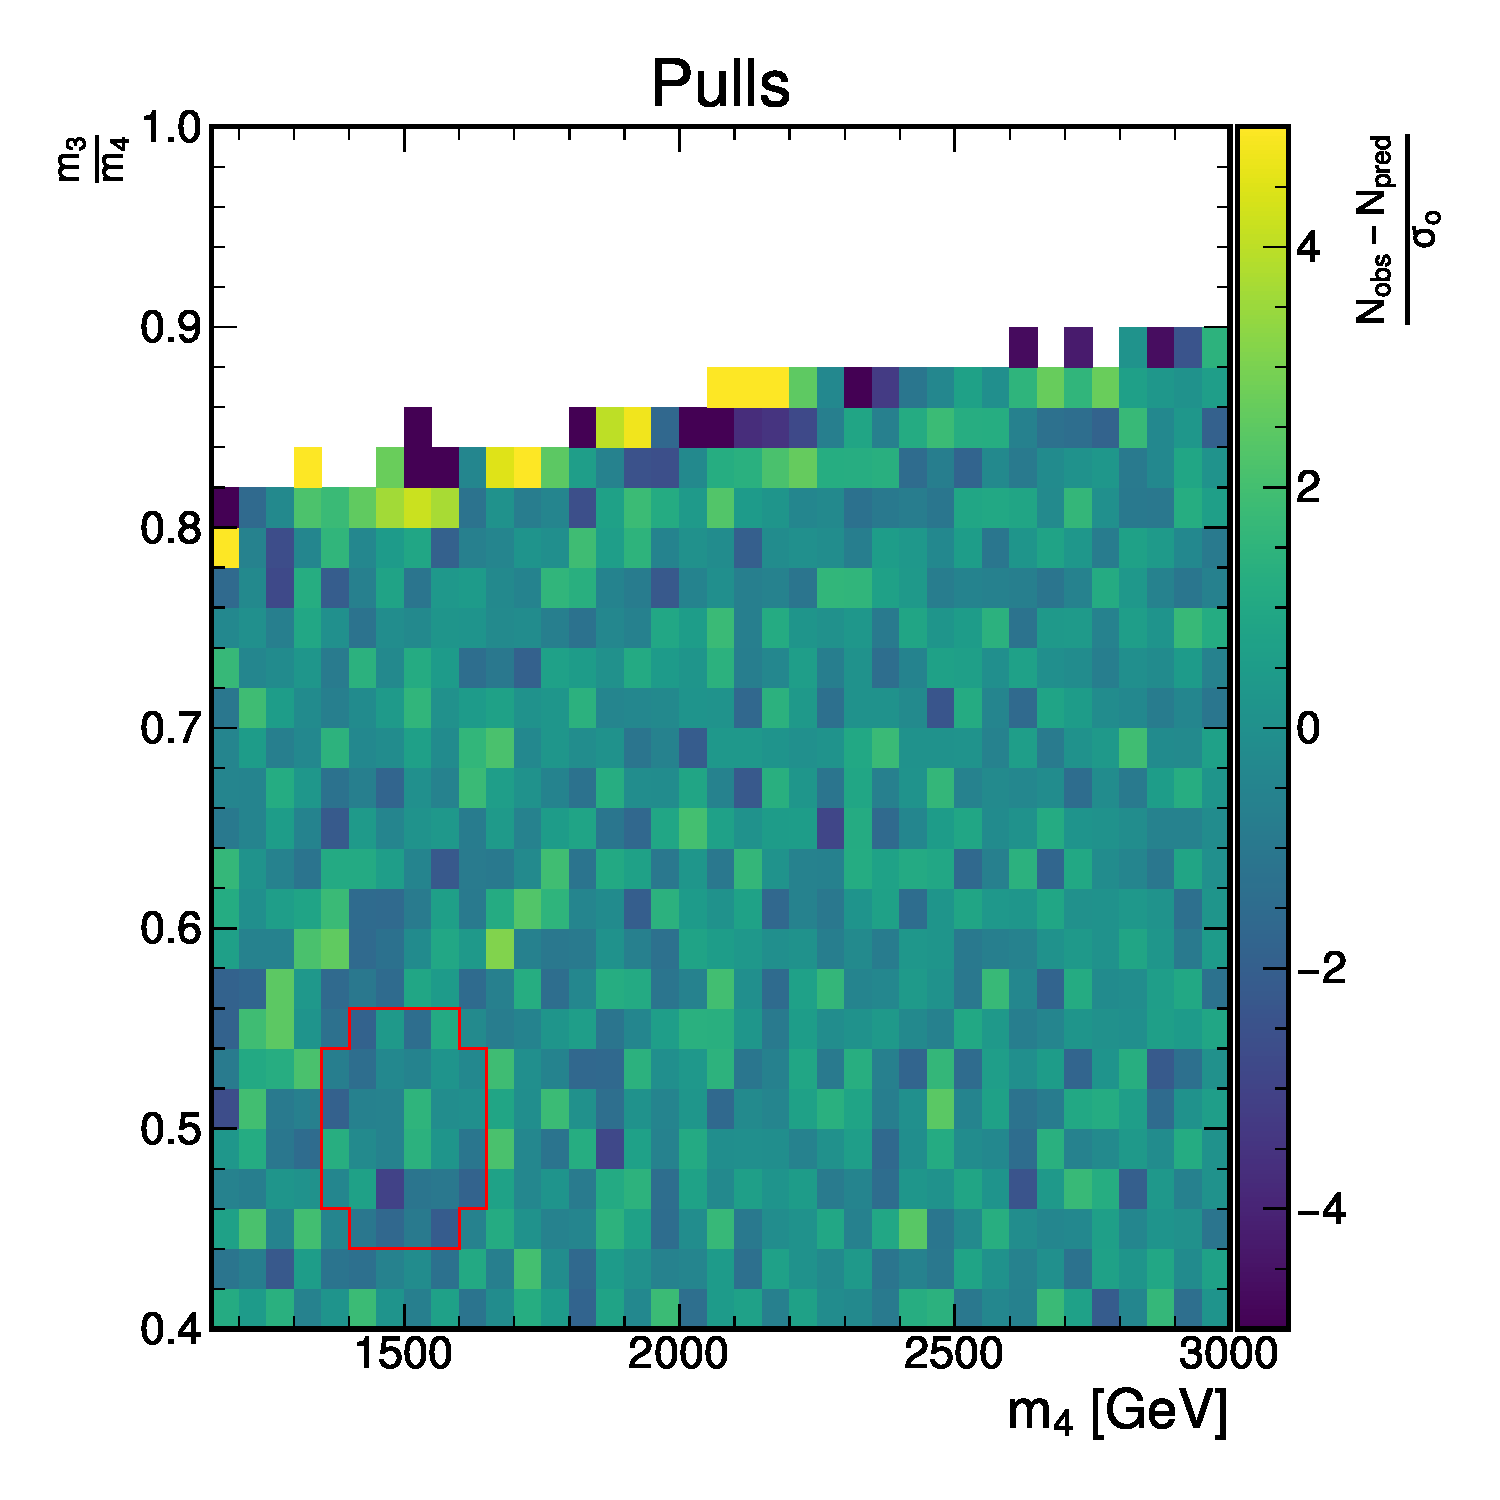
\includegraphics[width=0.3\textwidth]{figures/2dpullplots/grbf/E_1500_0p5_150_0p07.pdf} 
    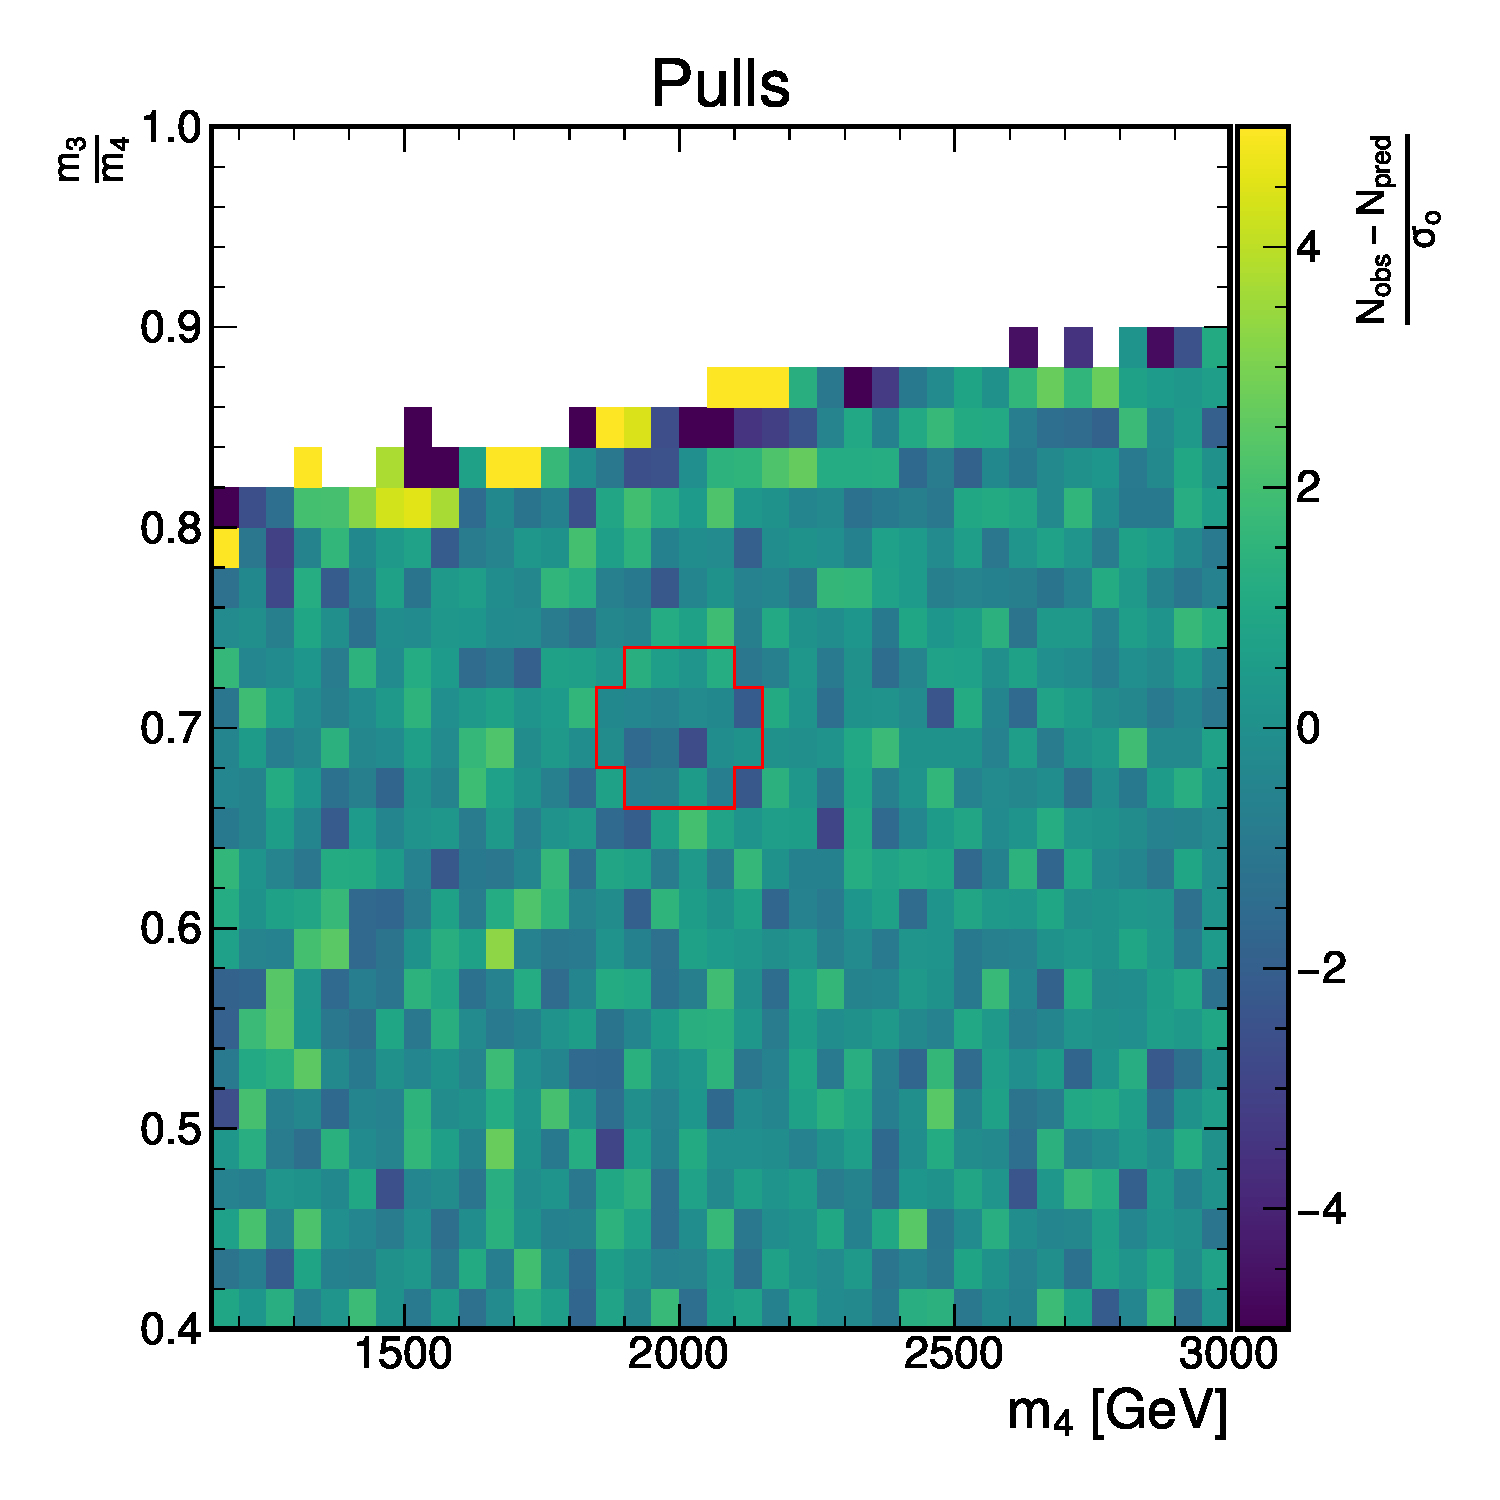
\includegraphics[width=0.3\textwidth]{figures/2dpullplots/grbf/E_2000_0p7_150_0p05.pdf} 
    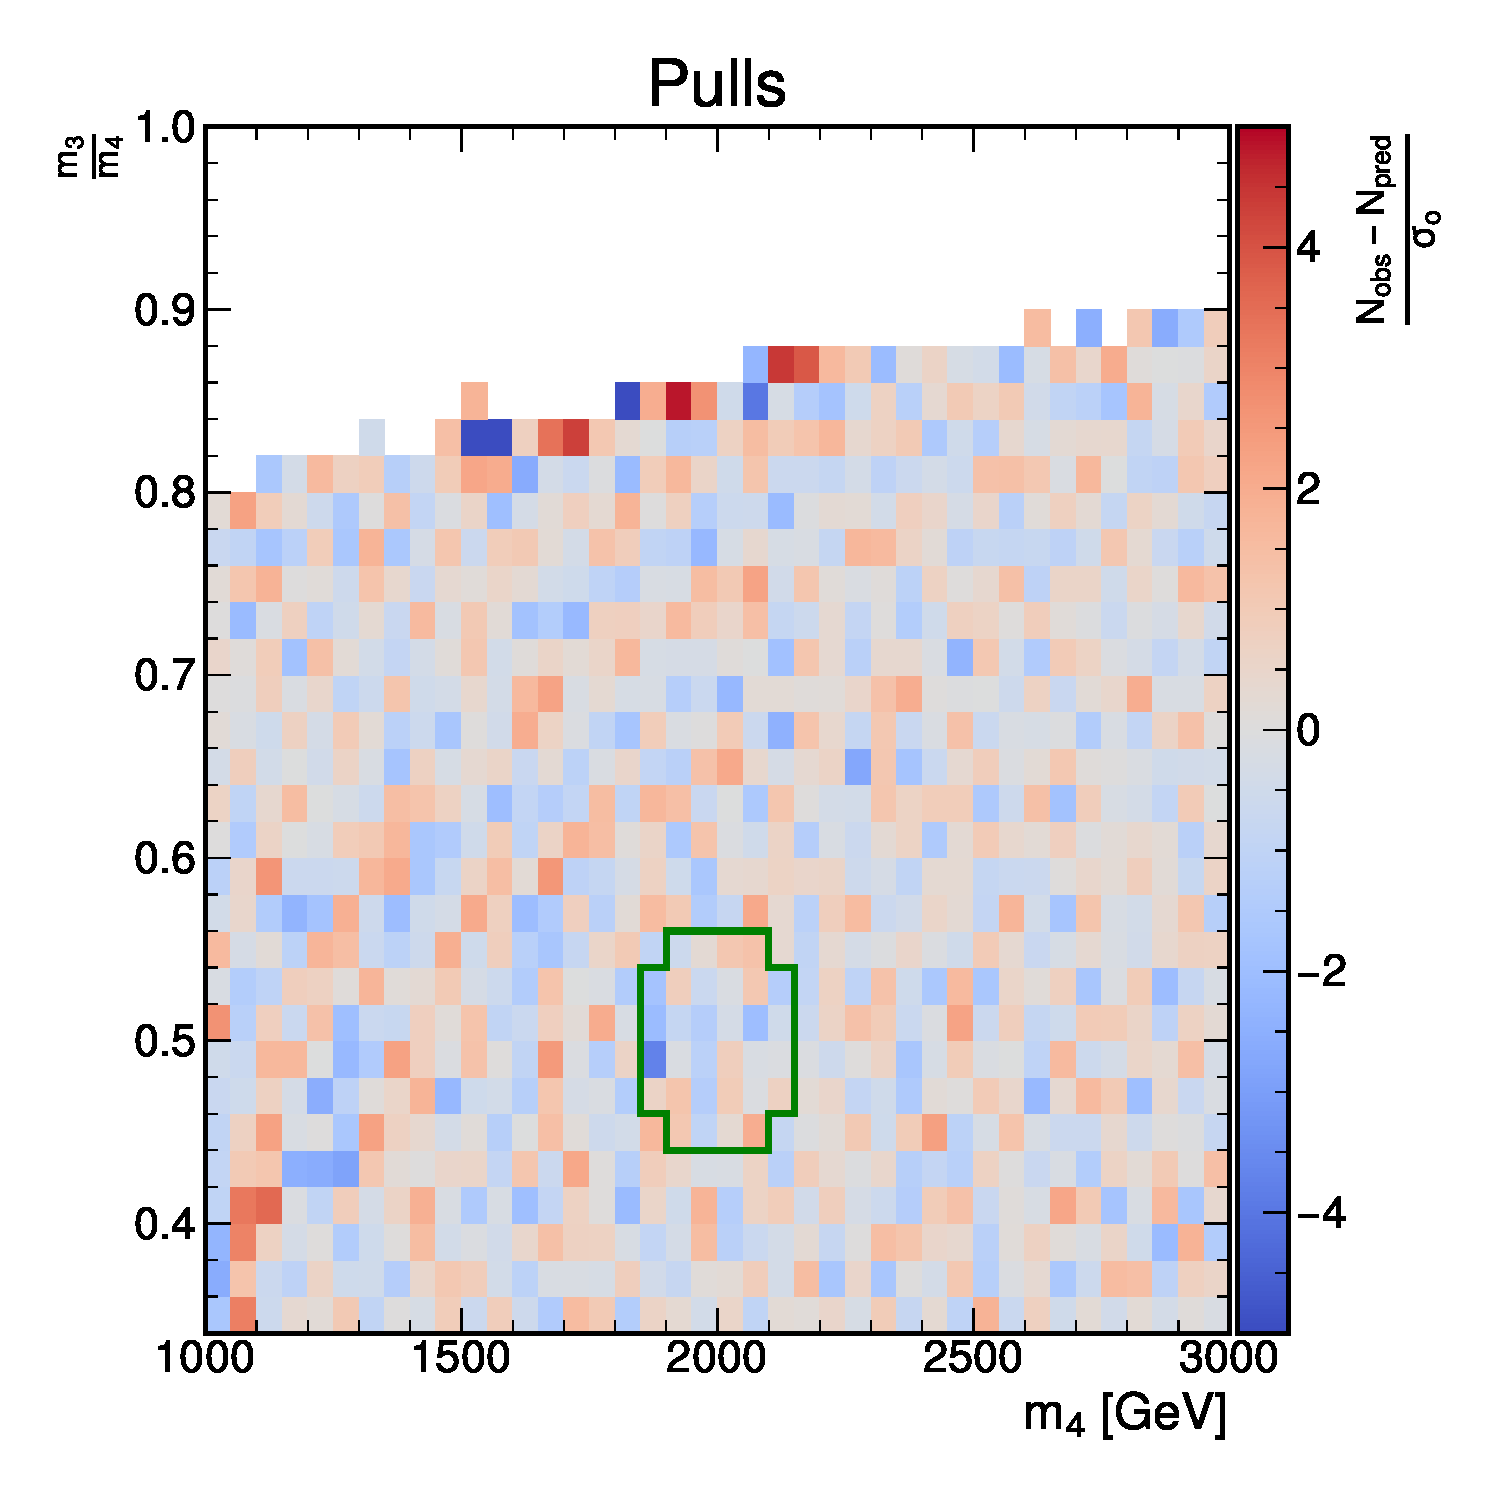
\includegraphics[width=0.3\textwidth]{figures/2dpullplots/grbf/E_2000_0p5_150_0p07.pdf} 
  \end{center}
\end{frame}

\begin{frame}{Fit Using Small Deep Kernel}
  \begin{center}
    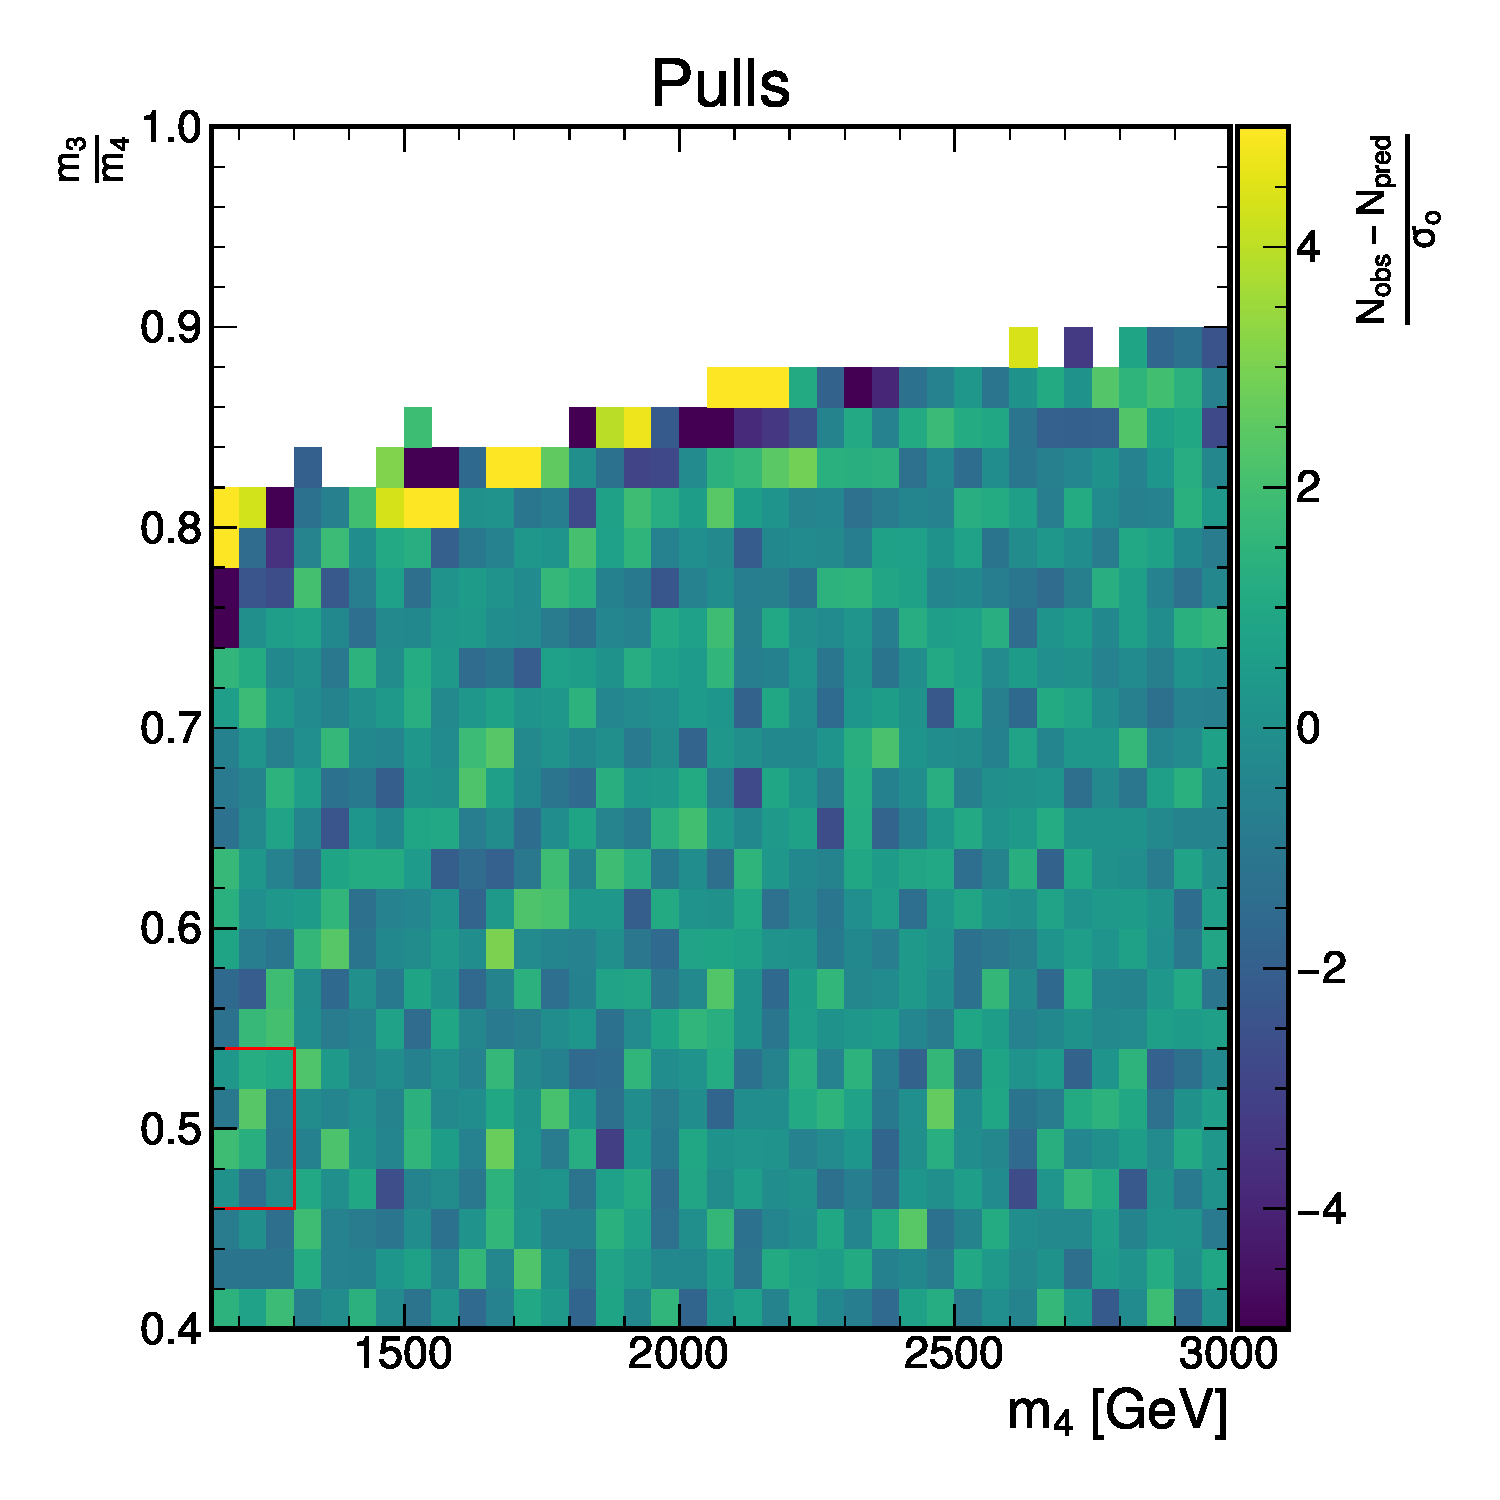
\includegraphics[width=0.3\textwidth]{figures/2dpullplots/nnrbf_16_8/E_1200_0p5_100_0p05.pdf} 
    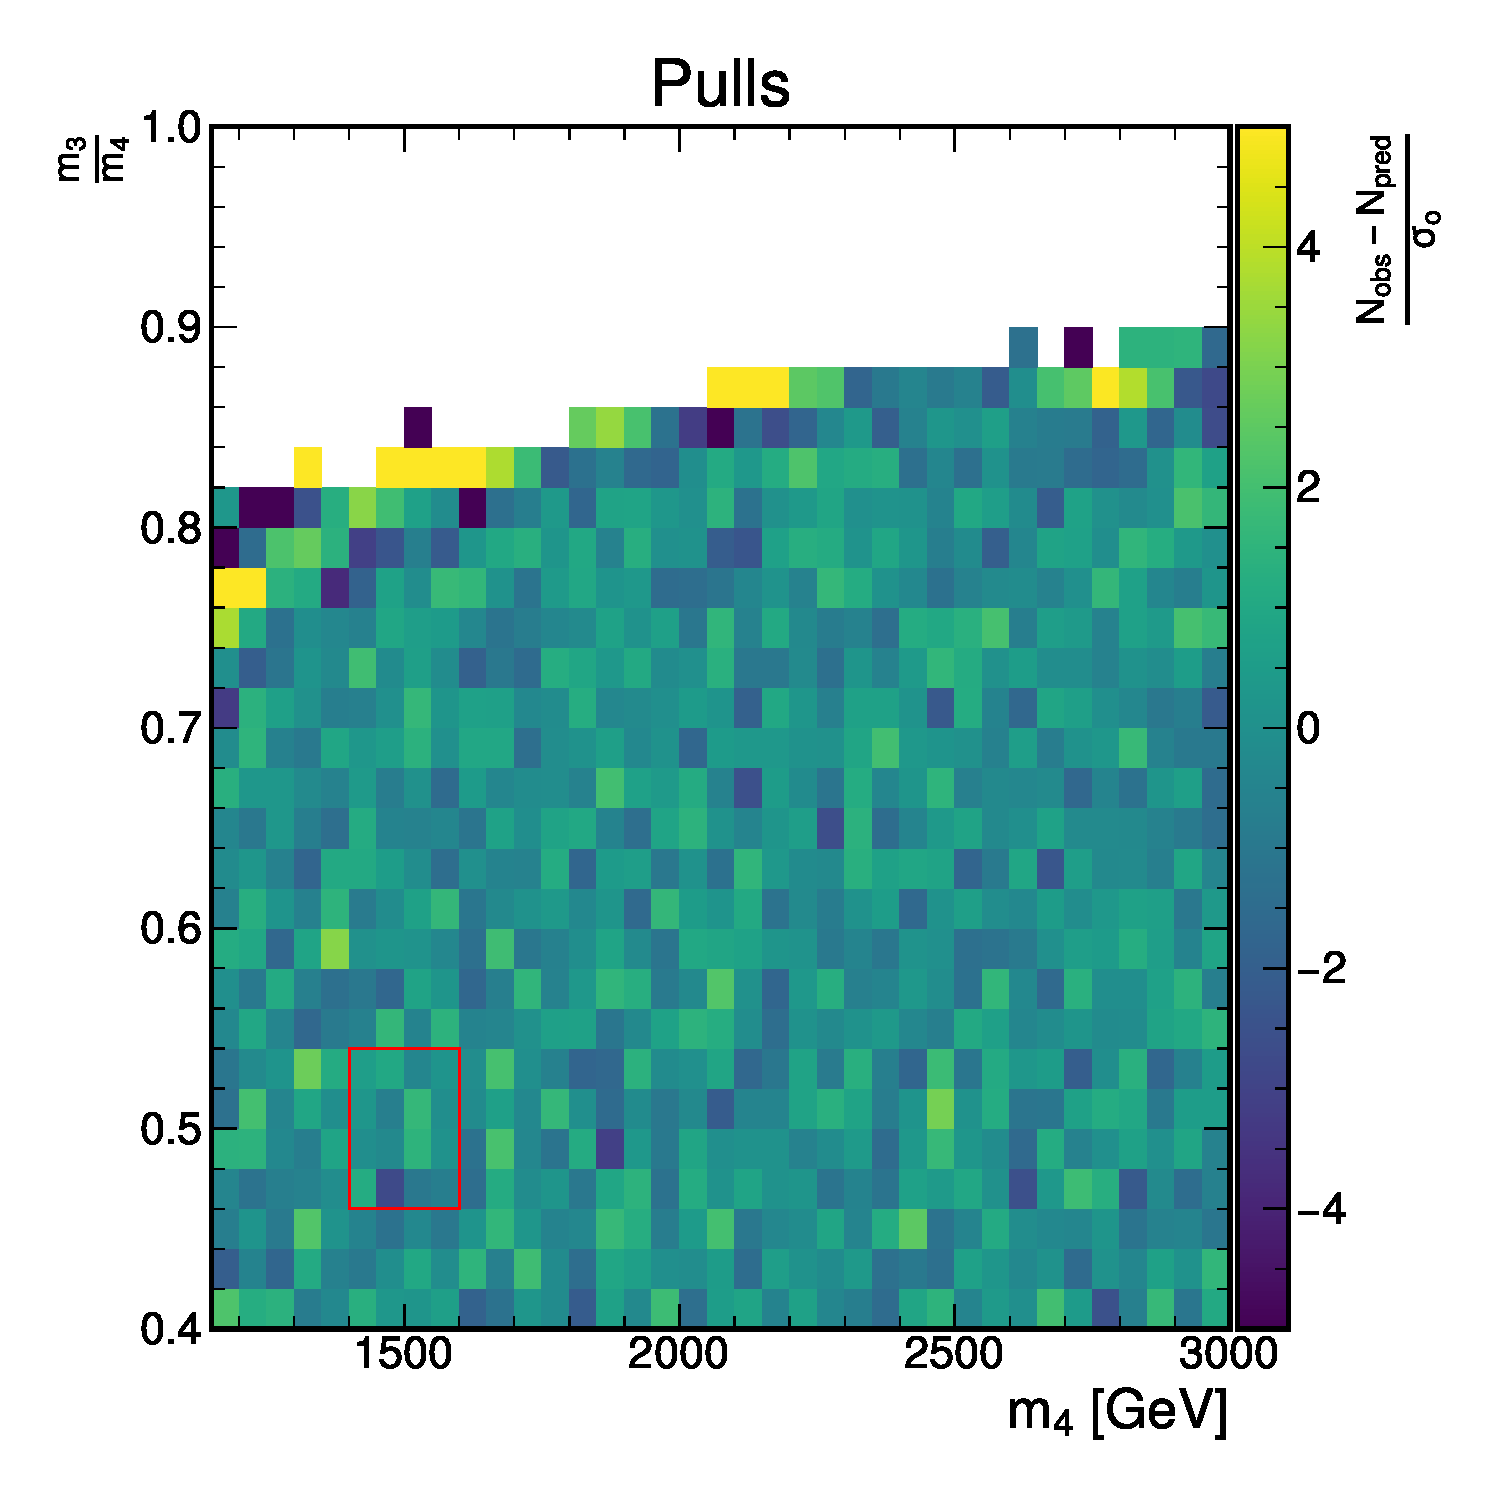
\includegraphics[width=0.3\textwidth]{figures/2dpullplots/nnrbf_16_8/E_1500_0p5_100_0p05.pdf} 
    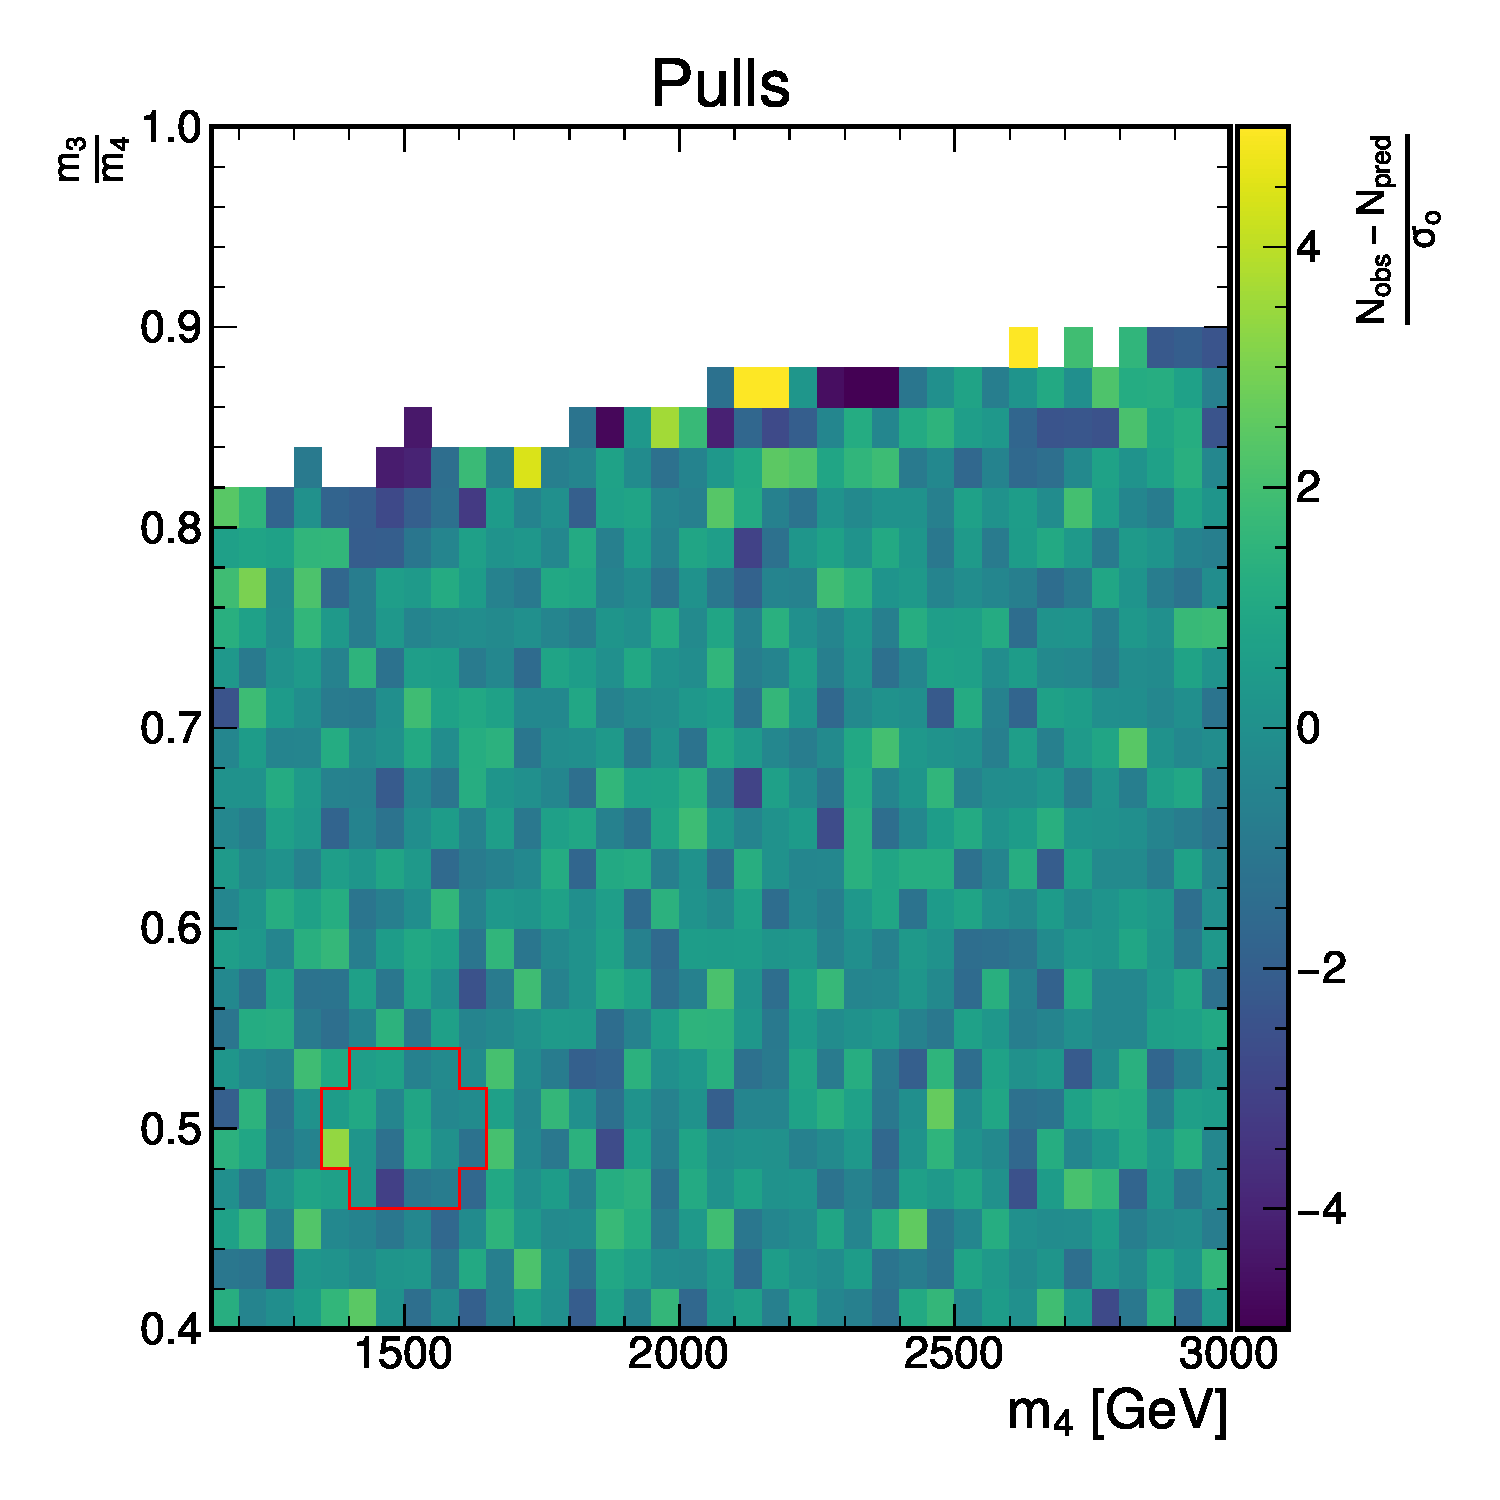
\includegraphics[width=0.3\textwidth]{figures/2dpullplots/nnrbf_16_8/E_1500_0p5_150_0p05.pdf} 
    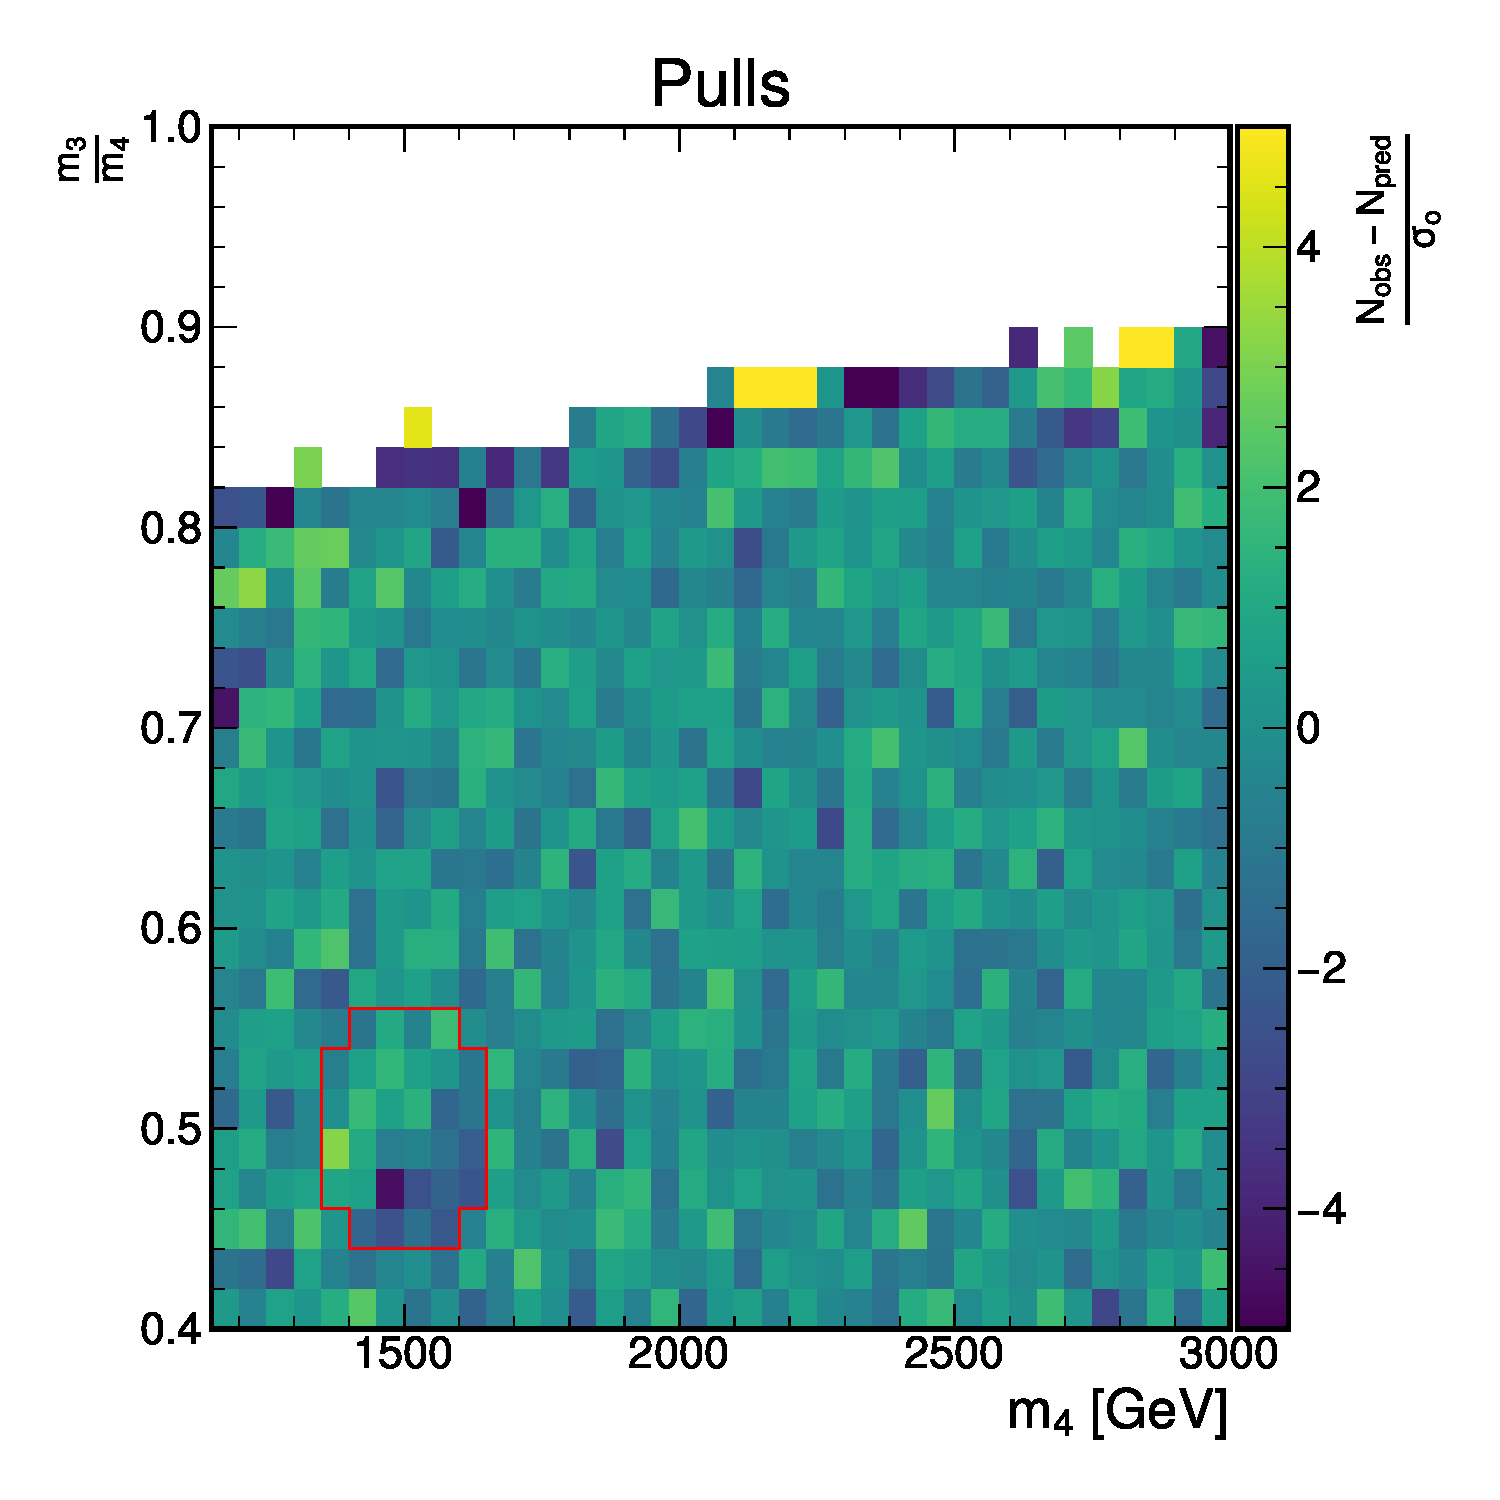
\includegraphics[width=0.3\textwidth]{figures/2dpullplots/nnrbf_16_8/E_1500_0p5_150_0p07.pdf} 
    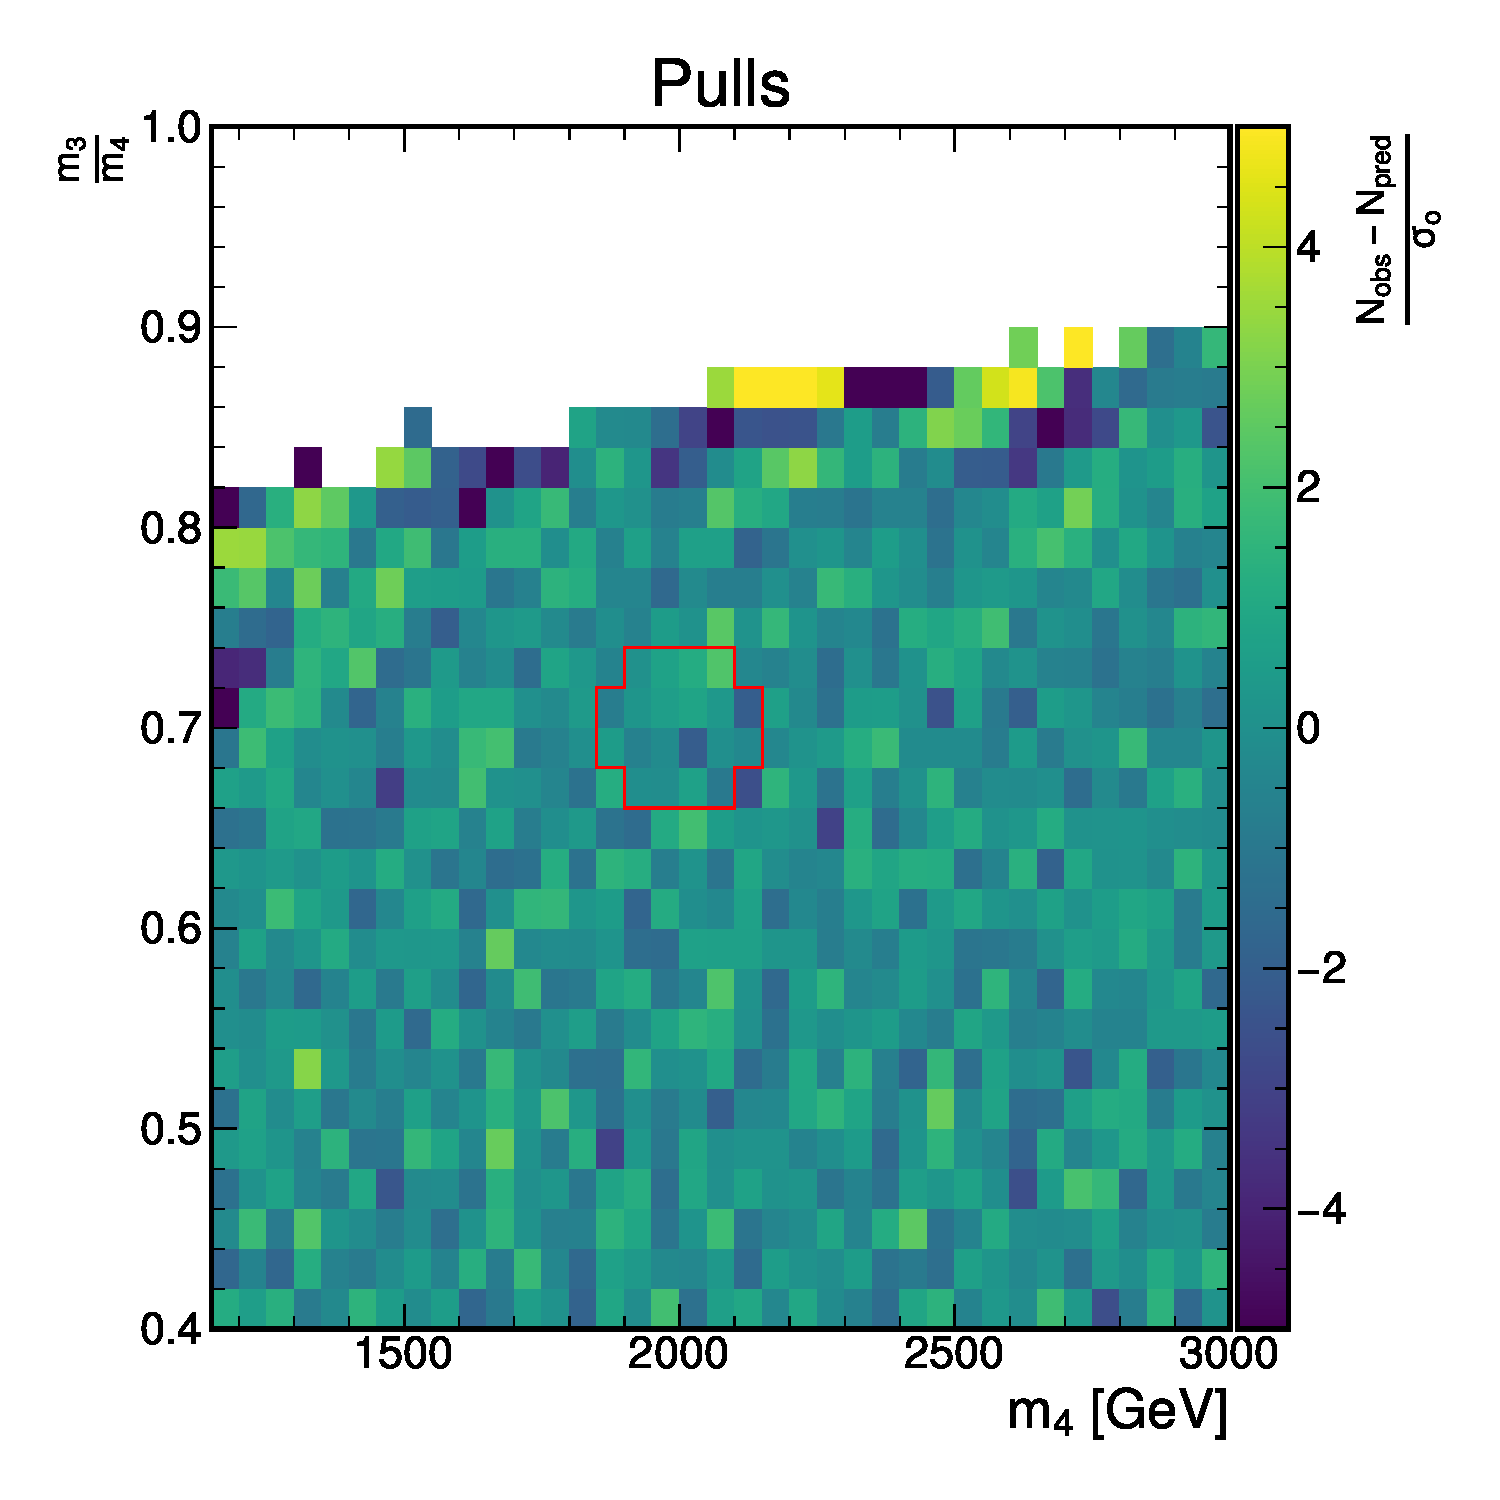
\includegraphics[width=0.3\textwidth]{figures/2dpullplots/nnrbf_16_8/E_2000_0p7_150_0p05.pdf} 
    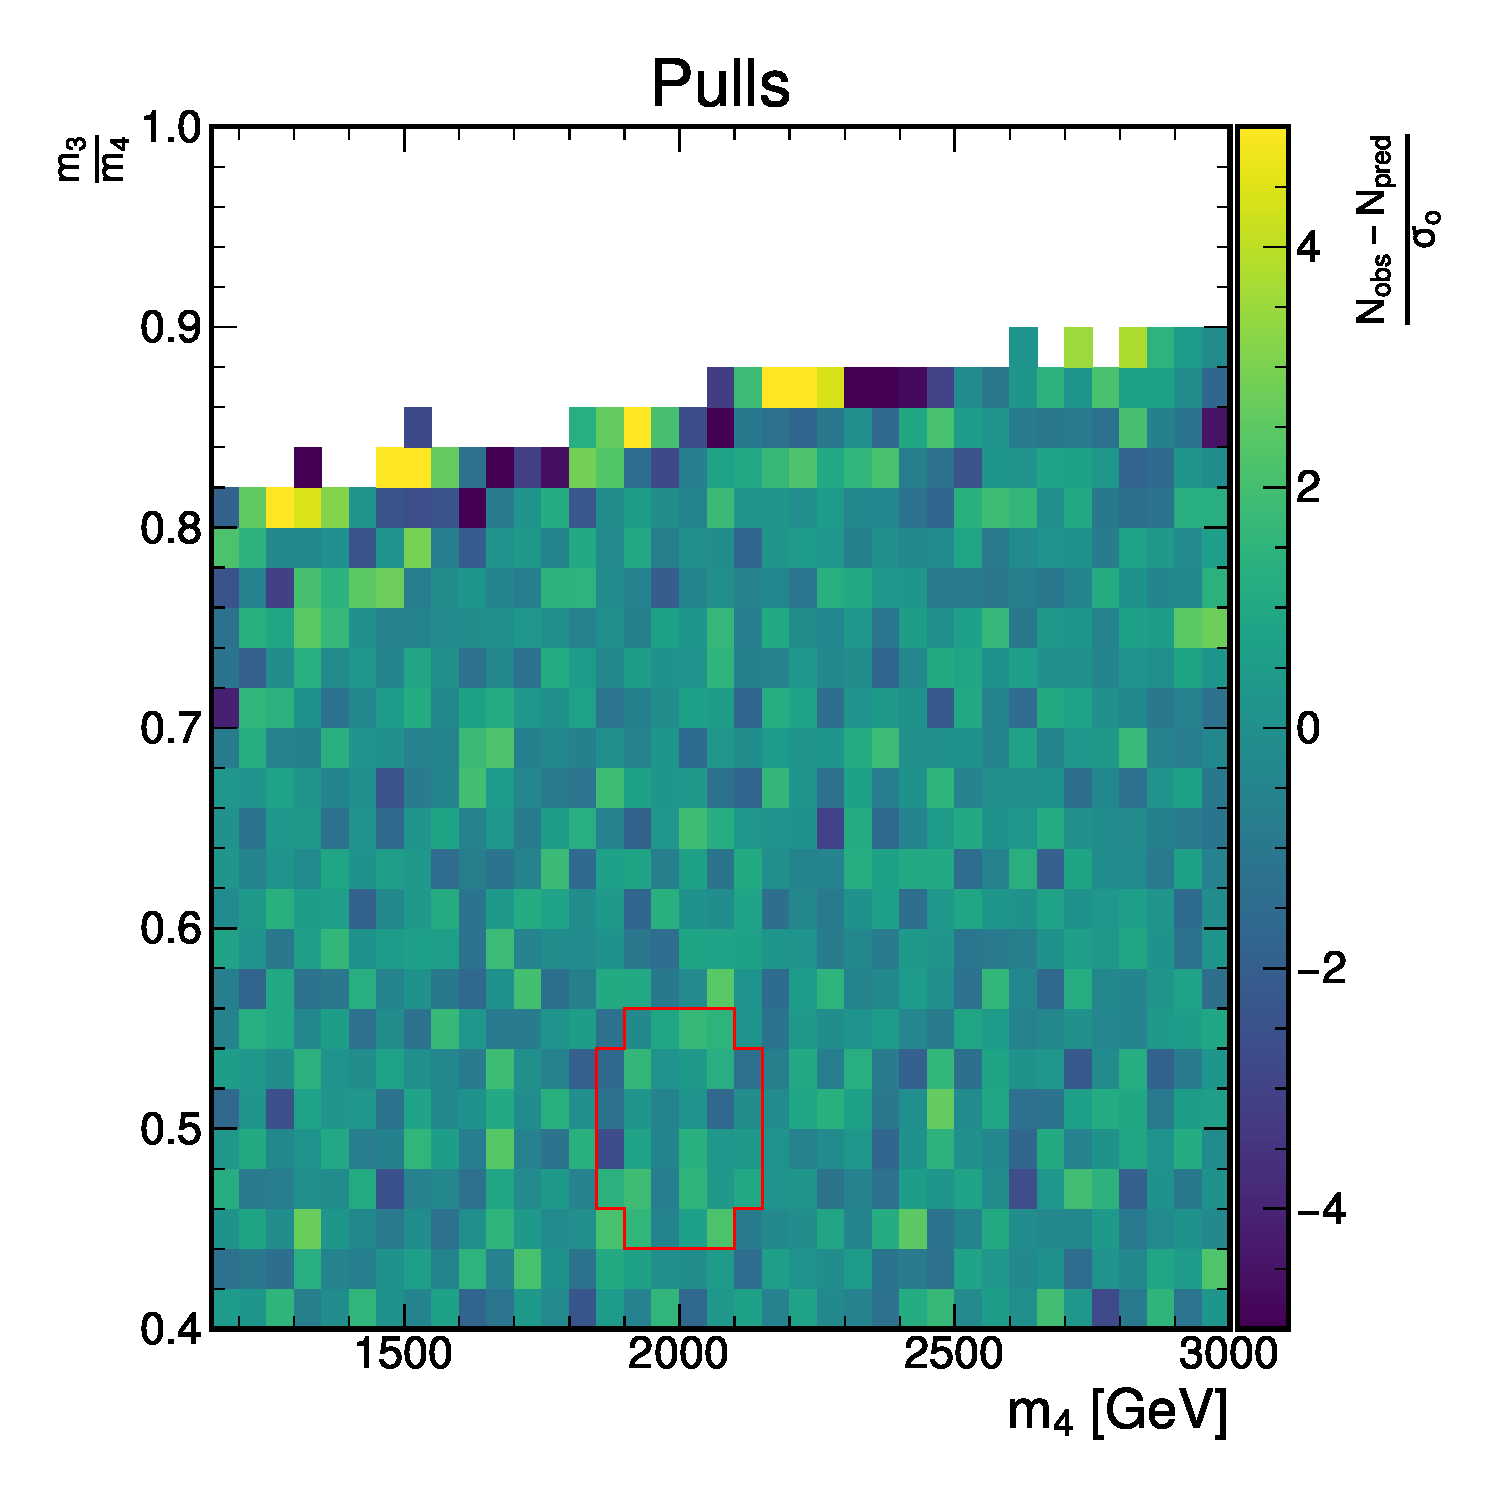
\includegraphics[width=0.3\textwidth]{figures/2dpullplots/nnrbf_16_8/E_2000_0p5_150_0p07.pdf} 
  \end{center}
\end{frame}

\begin{frame}{Fit Using Large Deep Kernel}
  \begin{center}
    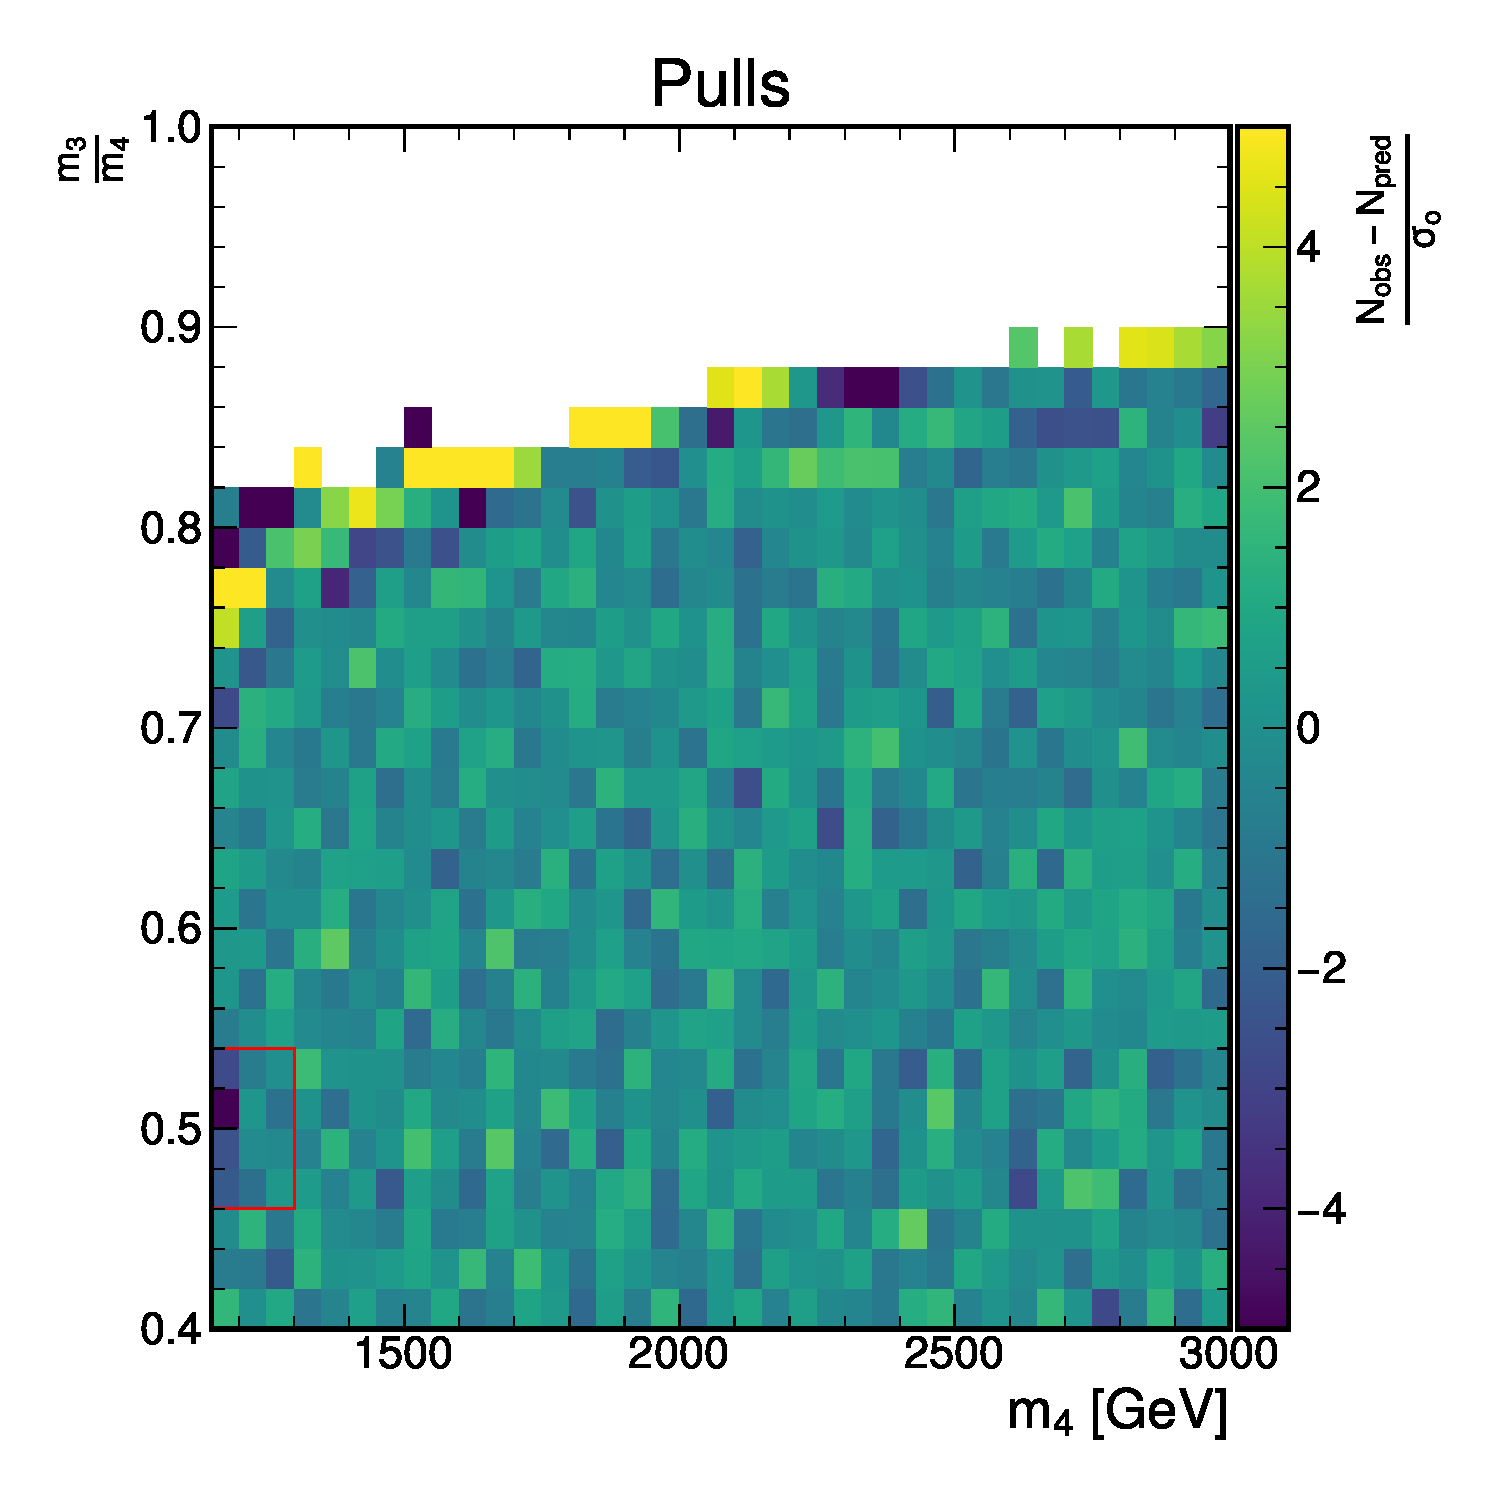
\includegraphics[width=0.3\textwidth]{figures/2dpullplots/nnrbf_256_128_16/E_1200_0p5_100_0p05.pdf} 
    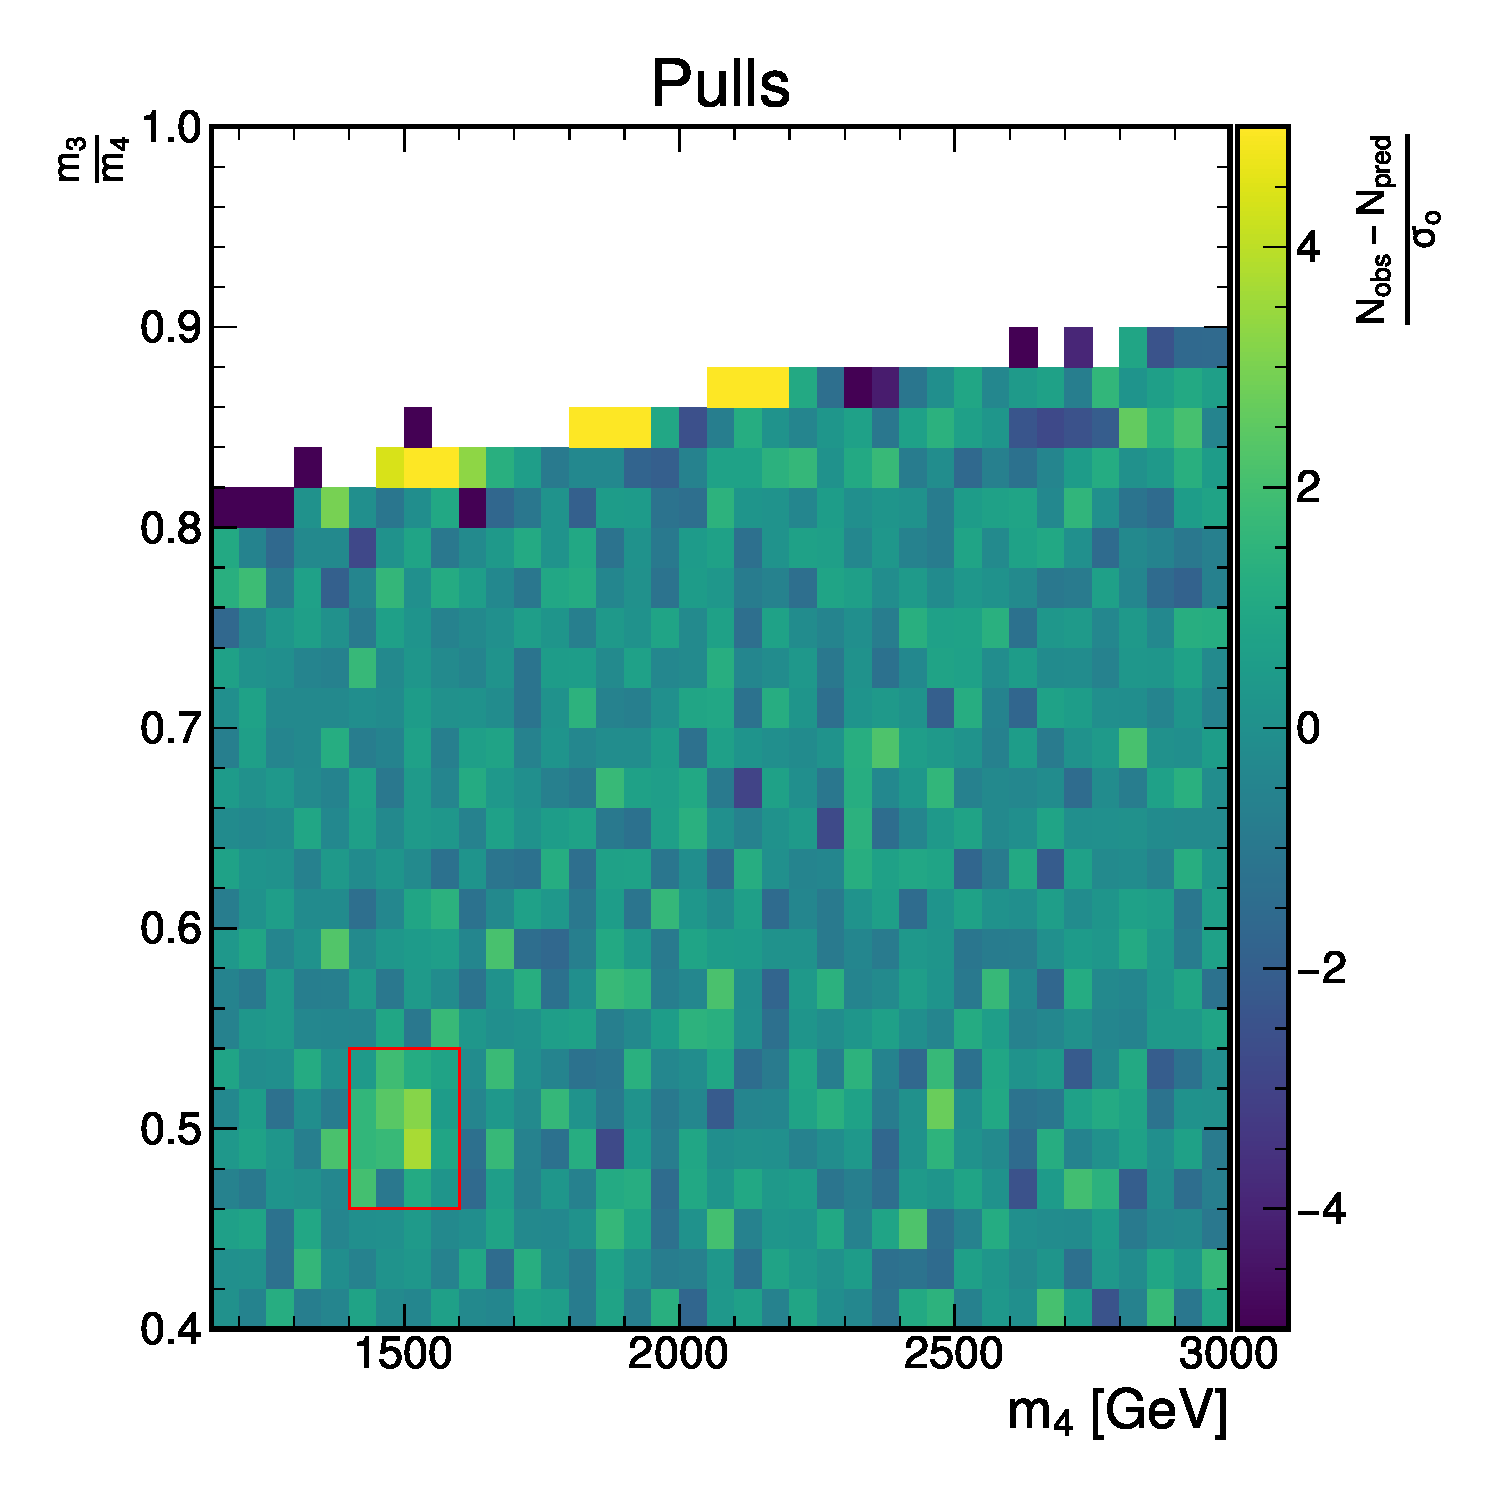
\includegraphics[width=0.3\textwidth]{figures/2dpullplots/nnrbf_256_128_16/E_1500_0p5_100_0p05.pdf} 
    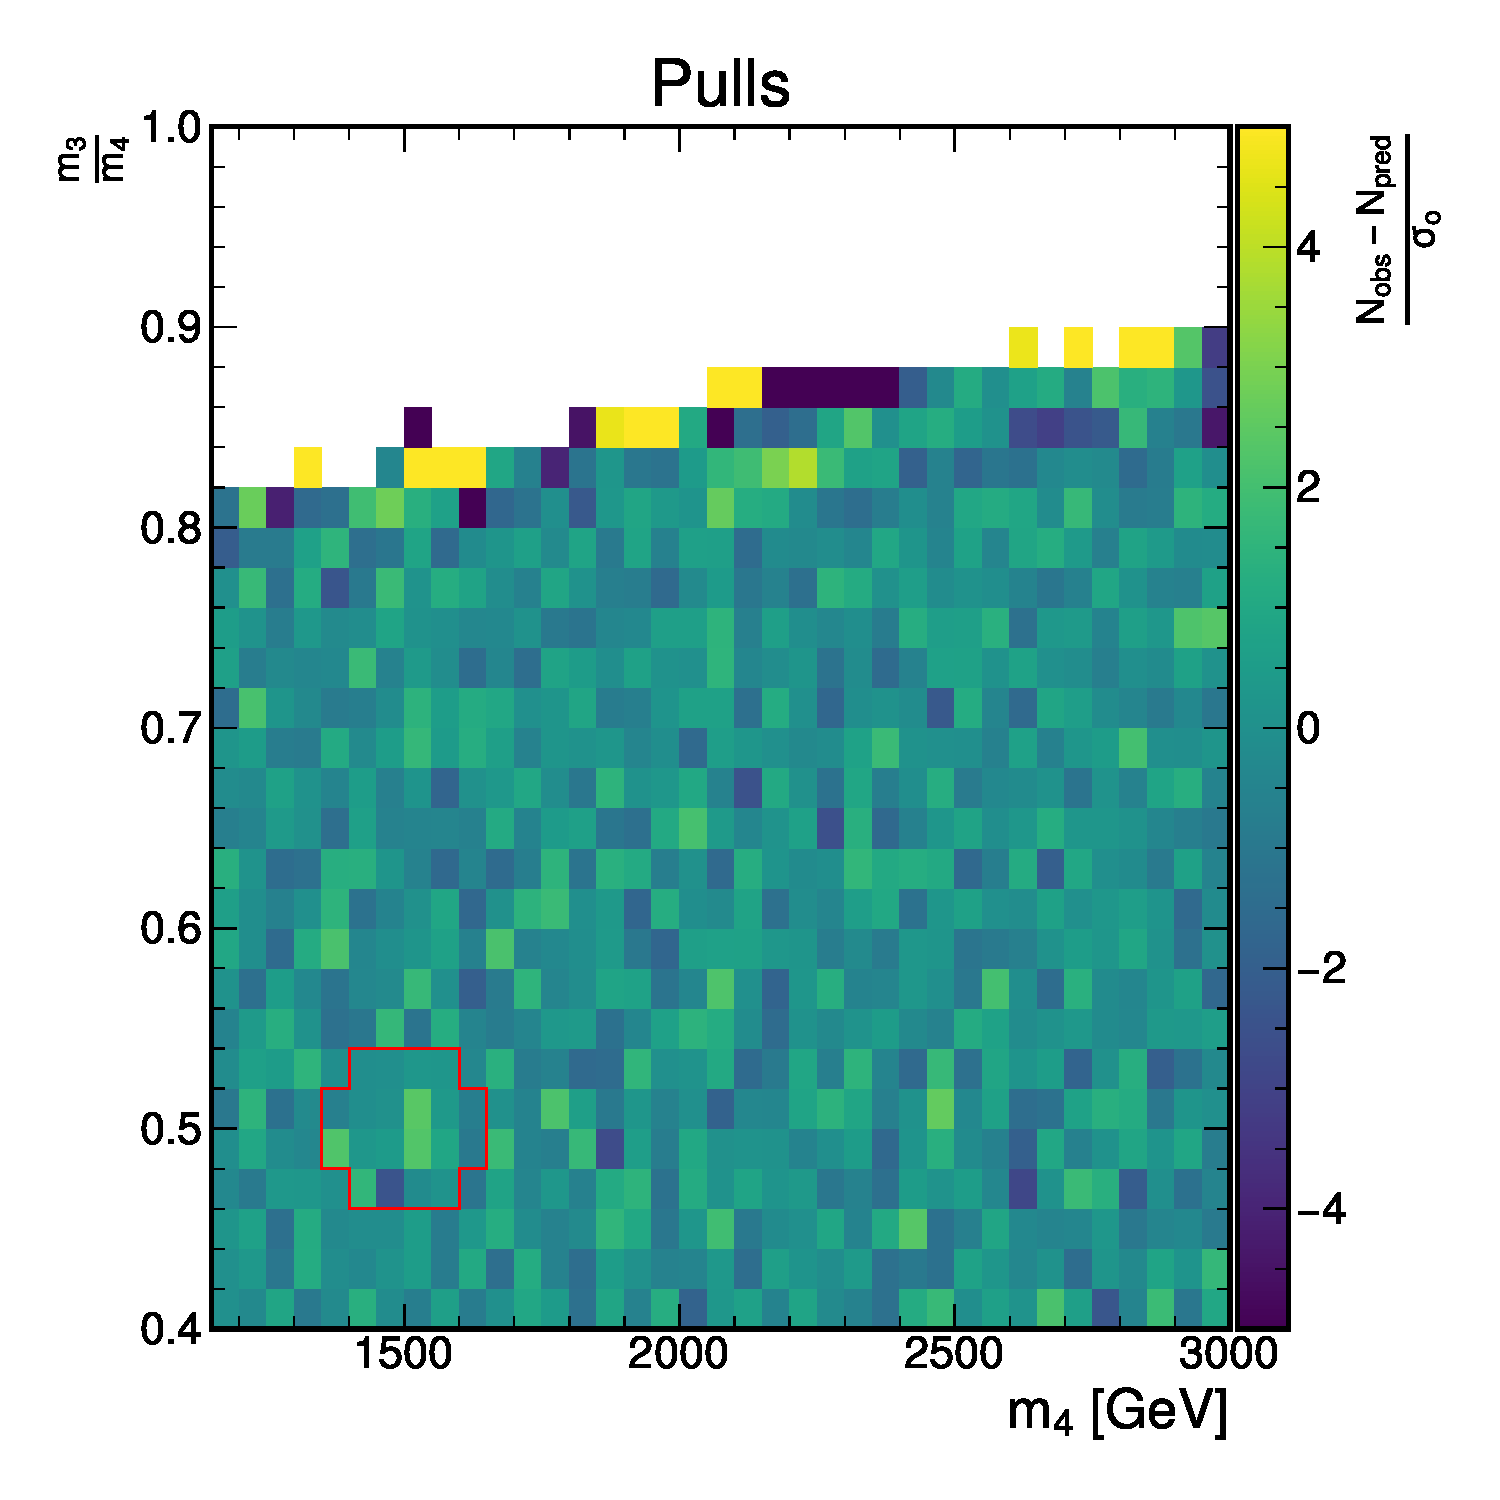
\includegraphics[width=0.3\textwidth]{figures/2dpullplots/nnrbf_256_128_16/E_1500_0p5_150_0p05.pdf} 
    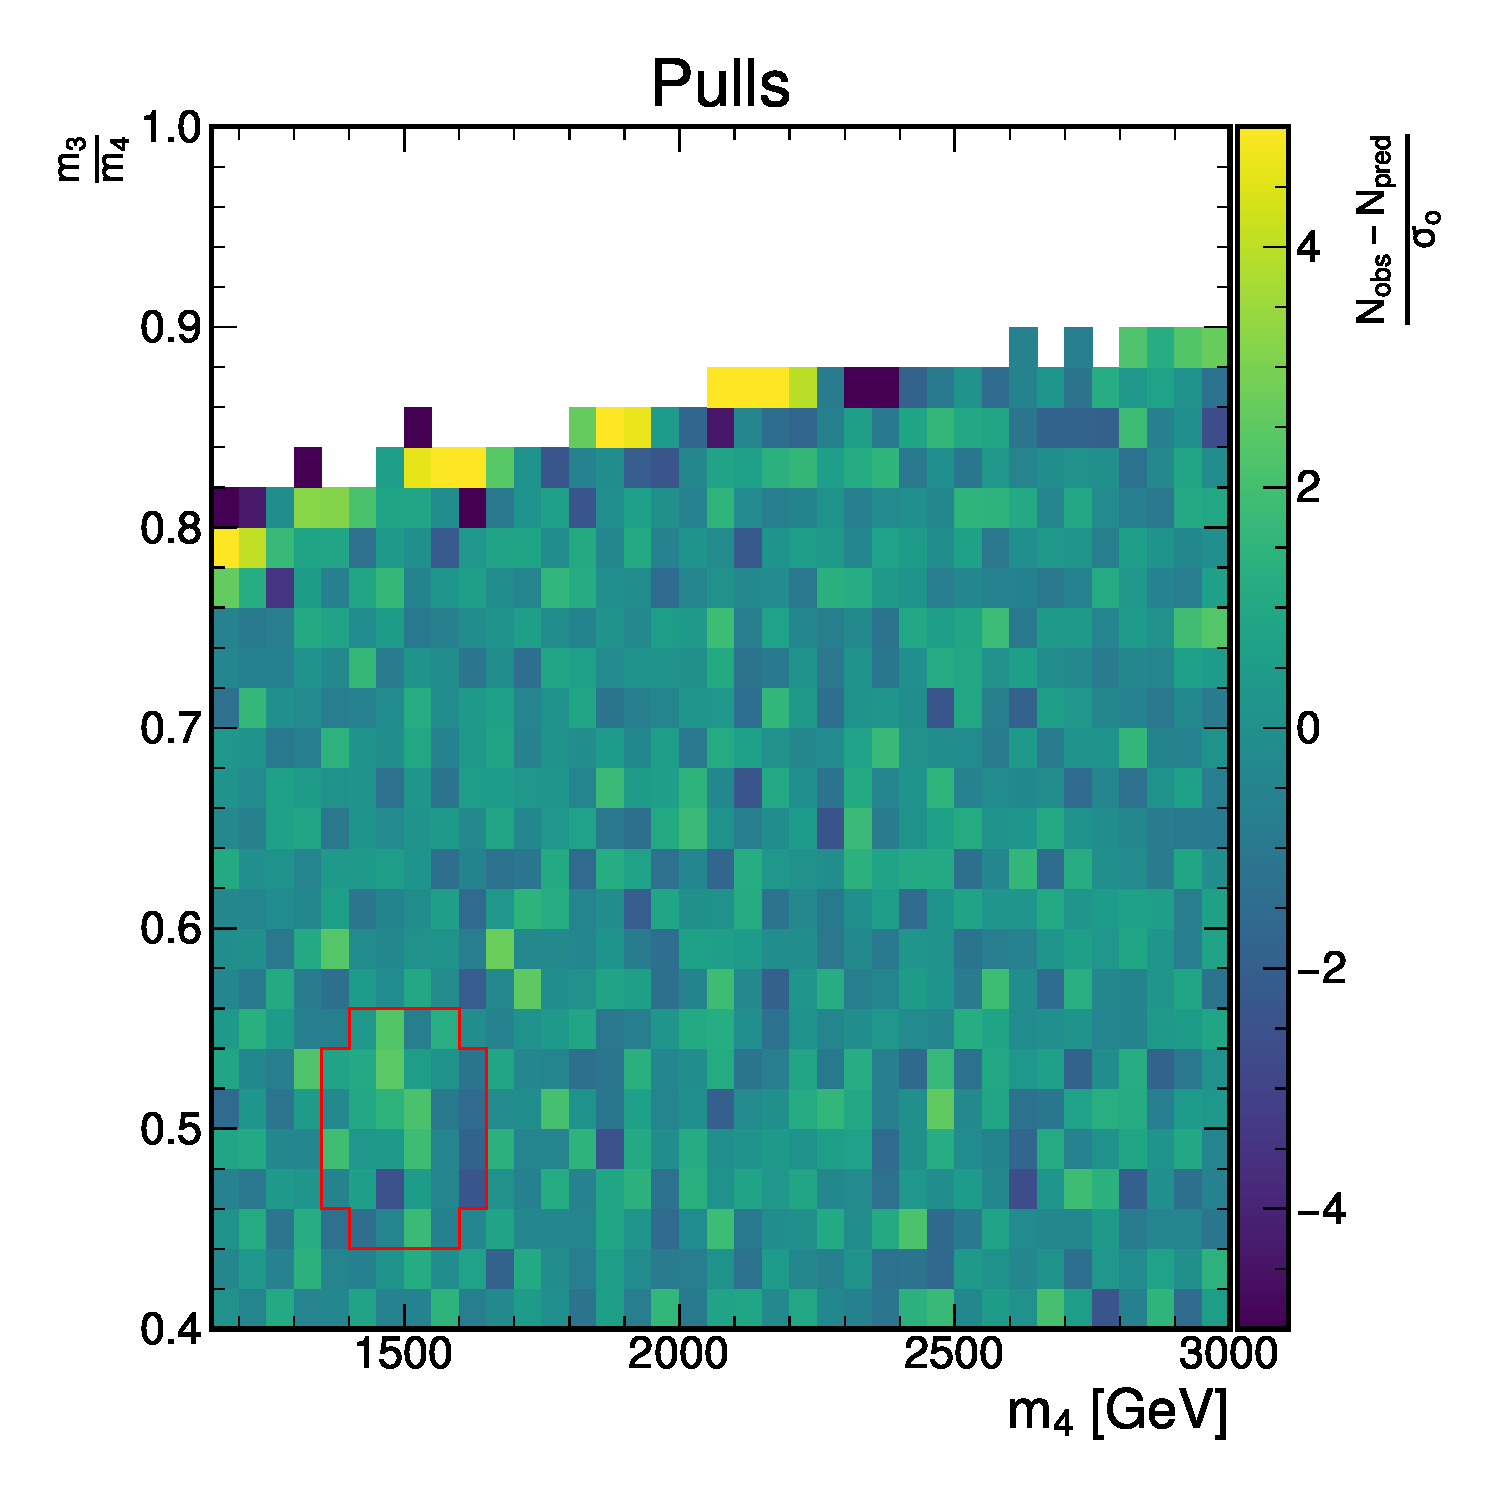
\includegraphics[width=0.3\textwidth]{figures/2dpullplots/nnrbf_256_128_16/E_1500_0p5_150_0p07.pdf} 
    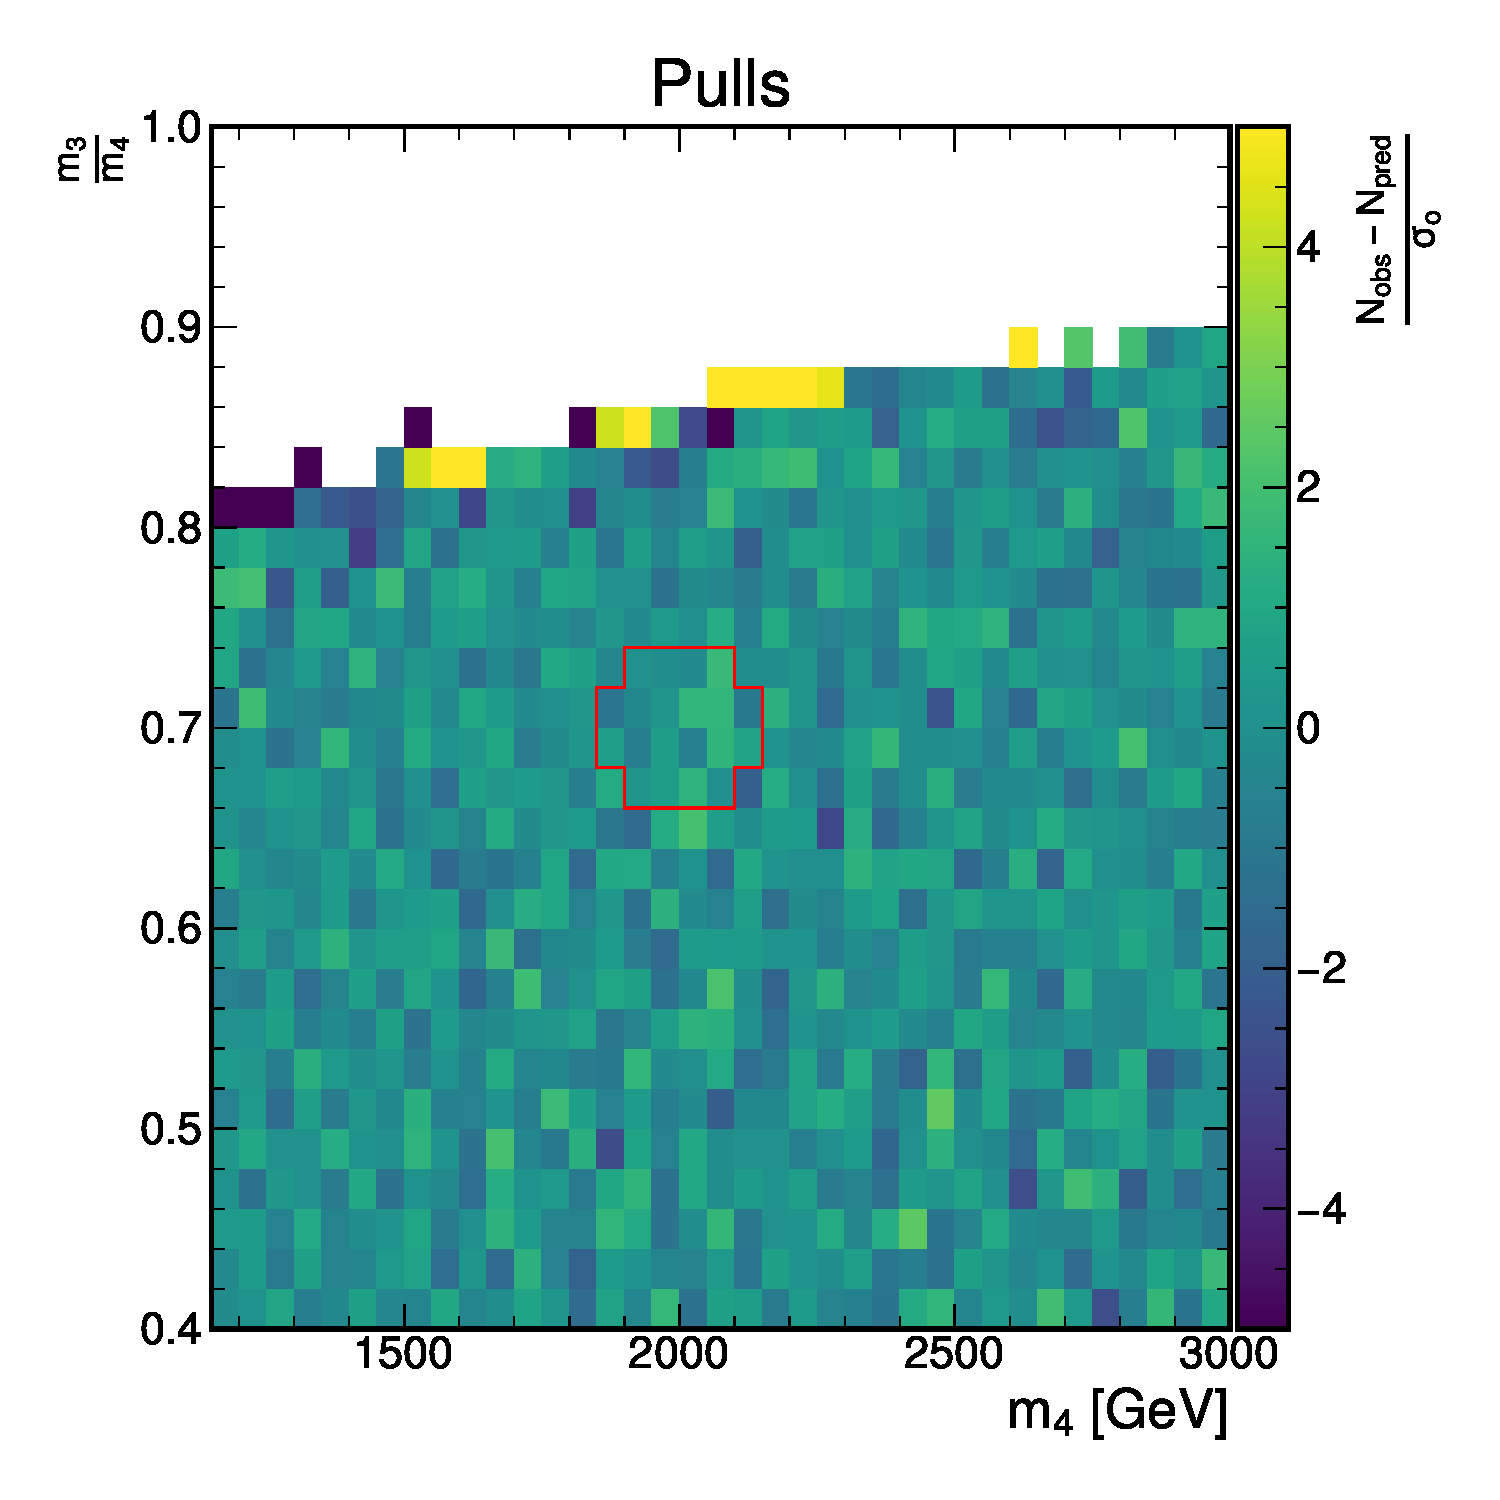
\includegraphics[width=0.3\textwidth]{figures/2dpullplots/nnrbf_256_128_16/E_2000_0p7_150_0p05.pdf} 
    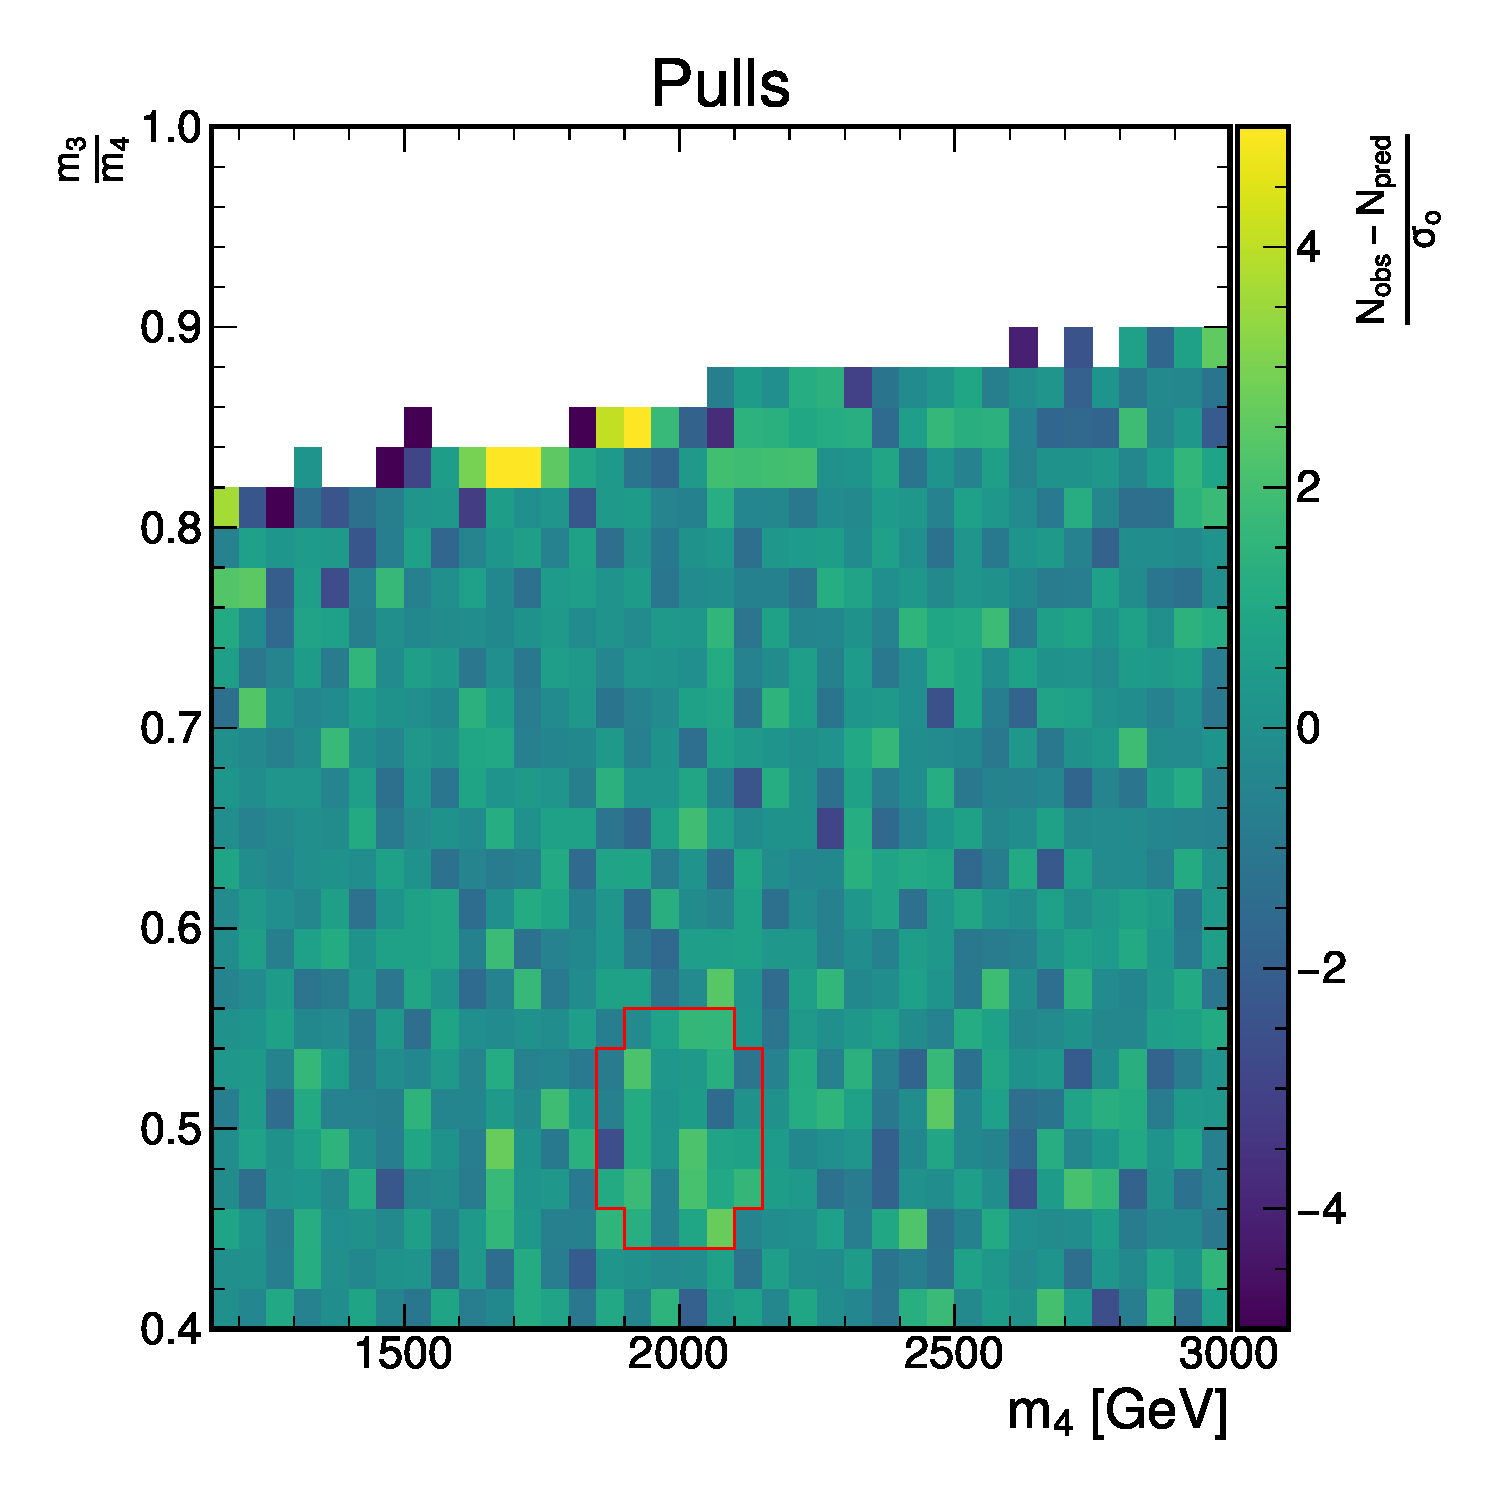
\includegraphics[width=0.3\textwidth]{figures/2dpullplots/nnrbf_256_128_16/E_2000_0p5_150_0p07.pdf} 
  \end{center}
\end{frame}


\section[Statistical Considerations]{Preliminary Statistical Strategy}

\begin{frame}{Notes on Statistical Procedure}
  \begin{itemize}
  \item Gaussian process regression provides a complete posterior distribution describing the background. 
  \item Therefore, a proper statistical treatment requires considering not just the posterior mean, but the complete distribution.
    \begin{itemize}
    \item We are working on an implementation in combine, using the eigenvectors of the posterior covariance as nuisance parameters templates. 
    \item MCMC/SVI can be externally using packages like pyro or emcee to build the statistical model directly in python.
    \end{itemize}
  \item {\bfseries This is is an area of active work. } However, we have made steady progress and have an ``alpha'' implementation.
  \end{itemize}


\end{frame}

% \begin{frame}{Systematic Uncertainties and Validation}
%   \begin{itemize}
%   \item We envision a validation strategy where the kernel hyperparameters are trained on SR data, then the regression is validated by examining the fit quality in simulation and CR data.
%   \item More work needed to determine exactly what systematics should be considered, and how they should be implemented.
%   \end{itemize}
%   
%   
%   SHOW COMPARISON OF CR AND MC 
% \end{frame}


\section{Conclusion}
\label{sec:conclusion}


\begin{frame}{Conclusion}
  \begin{itemize}
  \item The past months have seen substantial progress on the background estimation and statistical analysis procedure.
  \item Framework can now produce good estimates for 2D backgrounds over a range of locations and masking windows. Ongoing work on improving and unifying estimation. 
  \item We hope to present on further topics in the coming weeks, including trigger studies and data/mc comparisons, hopefully for Run3 as well. 
  \item We hope to hear any feedback from experts regarding the methodology, or any comments or suggestions!
  \end{itemize}
  \vspace{1cm}

  \begin{center}
    {\Large Thank you!}
  \end{center}
\end{frame}


\begin{frame}[allowframebreaks]{Bibliography}
  \bibliographystyle{plain}
  \bibliography{bibliography.bib}
\end{frame}


\appendix

\section{Appendix}
\label{sec:appendix}


\begin{frame}{Luminosity Issues}
  \relax
\end{frame}

\begin{frame}{Table of Common Kernels}
  \begin{center}
    \graphiccite{figures/kernel_table}{0.8}{rasmussen_gaussian_2006}
  \end{center}
  \begin{center}
    Some common kernels used in GPR. In the table, ``S'' indicates if the kernel is stationary, and ``ND'' indicates if the kernel is non-degenerate (does not have a finite number of nonzero eigenvalues).
  \end{center}
\end{frame}

\begin{frame}{Model Selection}
  \begin{itemize}
  \item The choice of kernel, both in terms of structure and hyperparameters, is referred to as model selection. 
  \item There is no one answer to model selection and in fact, it furnishes a deep opprotunity to learn about the problem.
    Generally requires a balance of rigor, numerical tractibility, and heuristics.  
  \item A true heirarchical model, were we define priors over models and apply Baye's rule repeatedly, is generally intractible.
  \item More often, we must use our knowkledge of the problem to select appropriate kernels. For example, knowing that the problem at hand is stationary, isotropic, smooth, etc. 
  \item The choice of hyperparameters is often done by marginalizing the evidence over the training data.
  \end{itemize}
\end{frame}

\begin{frame}{Function Distributions}
  Gaussian process allow us to define distributions over the space of functions. Given a gaussian process $\mathcal{GP} \left( m(x) , k(x,x') \right)$, and some function $h$, then
  \begin{equation}
    \mathbf{h} \sim N(m(X) , k(X,X))
  \end{equation}
  Given $n$ points in $\mathbb{R}^{k}$, the gaussian process defined a $n$ dimensional multivariate gaussian $\mathcal{N}$. If a function $h(x)$ has has values $h_1,h_2,...,h_{n}$ at those points, then
  \begin{equation}
    p \left( h \right) \sim \mathcal{N}(h_{1}, ..., h_{n})
  \end{equation}

  \begin{center}
    \graphiccite{figures/prior_and_conditioning}{0.7}{rasmussen_gaussian_2006}
  \end{center}
\end{frame}


\end{document}



% Local Variables:
% eval: (progn (setq process-environment (copy-sequence process-environment))
% (let* ( (basedir (file-name-directory (directory-file-name (file-name-directory (buffer-file-name)))))
% (texmfpath (file-name-concat  basedir "texmf"))
% )
% (setq-local TeX-style-path (append TeX-style-path  (directory-files-recursively texmfpath "auto" t)))
% (setq-local reftex-bib-path (list basedir))
% (setenv "TEXMFHOME" texmfpath )
% (setenv "BIBINPUTS" basedir ))
% )
% End:
